\documentclass[12pt]{article}

%Importation de package pour l'utilisation des accents
\usepackage[utf8]{inputenc}
\usepackage[T1]{fontenc}
%importation du package pour les maths
\usepackage{mathtools}
%importation du package pour les figures
\usepackage{graphicx}
%importation du package pour les citations
\usepackage{cite}
%importation du package pour réduire les marges
%\usepackage{fullpage}
%géométrie de la page
\usepackage{geometry}
 \geometry{a4paper,total={160mm,230mm},left=25mm,top=3.5cm}
%importation du package pour les url
\usepackage{hyperref}
%importantion package couleurs
\usepackage{color}
\usepackage{xcolor}
\usepackage{tcolorbox}
\usepackage{wrapfig}
\usepackage[french,english]{babel}
%Plusieurs colonnes
\usepackage{multicol}


\usepackage{amsmath}
\usepackage{listings}
\usepackage{pdflscape}
\usepackage{siunitx}

\usepackage{caption}
\usepackage{subcaption}
 
\definecolor{codegreen}{rgb}{0,0.6,0}
\definecolor{codegray}{rgb}{0.5,0.5,0.5}
\definecolor{codepurple}{rgb}{0.58,0,0.82}
\definecolor{backcolour}{rgb}{0.95,0.95,0.92}
 
\lstdefinestyle{mystyle}{
    backgroundcolor=\color{backcolour},   
    commentstyle=\color{codegreen},
    keywordstyle=\color{magenta},
    numberstyle=\tiny\color{codegray},
    stringstyle=\color{codepurple},
    basicstyle=\footnotesize,
    breakatwhitespace=false,         
    breaklines=true,                 
    captionpos=b,                    
    keepspaces=true,                 
    numbers=left,                    
    numbersep=5pt,                  
    showspaces=false,                
    showstringspaces=false,
    showtabs=false,                  
    tabsize=2
}

\lstset{style=mystyle}


\definecolor{light-gray}{gray}{0.95}
\newcommand{\code}[1]{\colorbox{light-gray}{\parbox{0.9\textwidth}{\texttt{\small{#1}}}}}



% définition du style des pages pour l'entête et les pieds de pages
\usepackage{fancyhdr}
\pagestyle{fancy}
\setlength{\headheight}{15pt}
% configuration des pieds de pages:
% trait entre les pieds de pages et le texte de la page.
\renewcommand{\footrulewidth}{1pt}
% configuration des hauts de pages:
% trait entre l'entête et le texte de la page
\renewcommand{\headrulewidth}{1pt} 
% contenus aux positions L and R pour l'entête
\fancyhead[L]{\leftmark}
\fancyhead[R]{}
% contenus aux positions L and R:
\fancyfoot[L]{Carmelo Mileto $\&$ Eliott Johnson}
\fancyfoot[R]{\today}
\setlength{\baselineskip}{2\baselineskip}
\addtolength{\skip\footins}{1pc plus 5pt}

\usepackage{silence}
\WarningFilter{latex}{Text page 22 contains only floats}

\begin{document}
\selectlanguage{french}

\begin{titlepage}

\newcommand{\HRule}{\rule{\linewidth}{0.5mm}} % Defines a new command for the horizontal lines, change thickness here

\center % Center everything on the page
 
%----------------------------------------------------------------------------------------
%	HEADING SECTIONS
%----------------------------------------------------------------------------------------

\textsc{\LARGE Université de Genève}\\[1.5cm] % Name of your university/college
\textsc{\Large Master en Physique}\\[0.5cm] % Major heading such as course name
\textsc{\large Travaux Pratiques IV}\\[0.5cm] % Minor heading such as course title

%----------------------------------------------------------------------------------------
%	TITLE SECTION
%----------------------------------------------------------------------------------------

\HRule \\[0.4cm]
{ \huge \bfseries Temps de vie et flux des muons cosmiques}\\[0.4cm] % Title of your document
\HRule \\[1.5cm]
 
%----------------------------------------------------------------------------------------
%	AUTHOR SECTION
%----------------------------------------------------------------------------------------

\begin{minipage}{0.4\textwidth}
\begin{flushleft} \large
\emph{Auteur:}\\
E. \textsc{Johnson}, C. \textsc{Mileto} % Your name
\end{flushleft}
\end{minipage}
~
\begin{minipage}{0.4\textwidth}
\begin{flushright} \large
\emph{Superviseurs:} \\
A. \textsc{Bravard}, E. \textsc{Zaffaroni}
\end{flushright}
\end{minipage}\\[2cm]

% If you don't want a supervisor, uncomment the two lines below and remove the section above
%\Large \emph{Author:}\\
%John \textsc{Smith}\\[3cm] % Your name

%----------------------------------------------------------------------------------------
%	DATE SECTION
%----------------------------------------------------------------------------------------

{\large \today}\\[2cm] % Date, change the \today to a set date if you want to be precise

%----------------------------------------------------------------------------------------
%	LOGO SECTION
%----------------------------------------------------------------------------------------

\includegraphics[width=10cm]{Images/logos/physique_logo.png}\\[1cm] % Include a department/university logo - this will require the graphicx package
 
%----------------------------------------------------------------------------------------

\vfill % Fill the rest of the page with whitespace

\end{titlepage}



%pagenumbering permet de ne pas afficher le numéro en bas de page
\pagenumbering{gobble}


\tableofcontents
\newpage
%pagenumbering vas recommencer à numéroter en bas de page
\pagenumbering{arabic}


\begin{abstract}

La plupart des particules observées en dehors de notre atmosphère ont été crées par des sources galactiques, voir extra-galactiques. Si leurs énergies dépassent le  keV, celles-ci vont alors heurter la terre. La plupart des rayons cosmiques sont de nature hadronique et donc sensitif à l'interaction forte. L'atmosphère terrestre est alors un vrai champ de mine pour ces particules qui sont susceptible d'interagir à tout moment produisant des gerbes de particules neutres et chargées. Puis, à leur tour interagissent résultant en une pléthore de mésons chargées avec des temps de vie court qui éventuellement se désintègrent en énormément de muons de hautes énergies. À la surface de la terre, nous sommes bombardés par des muons de charges positive et négative avec un taux d'environ une particule par \si{\cm\squared\per\min}. Dans cette expérience, nous allons nous intéresser à  ces particules cosmiques et nous allons mesurer leurs temps de vie et leurs flux.

\end{abstract}

\newpage
\section{Calcul du temps de vie du muon}
%%%%%%%%%%%%%%%%%%%%%%%%%%%%%%%%%%%%%%%%%%%%%%%%%%%%%%%%%%%%%%%%%
%%% INTRODUCTION %%%%%%%%%%%%%%%%%%%%%%%%%%%%%%%%%%%%%%%%%%%%%%%%%%%%%%
%%%%%%%%%%%%%%%%%%%%%%%%%%%%%%%%%%%%%%%%%%%%%%%%%%%%%%%%%%%%%%%%%
\subsection{Théorie}

Les muons sont produit par la propagation des rayons cosmiques qui entrent dans l'atmosphère de la terre. Ce sont des particules élémentaires appartenant à la famille des leptons. Il y a 6 type de leptons: les électrons, les muons, les taus ainsi qu'un neutrino associé à chacune de ces particules. Les muons sont bien plus massifs que les électrons et sont capable d'atteindre le sol. Ce sont des particules de spin $\frac{1}{2}$ avec une masse au repos de m $=105.6$ MeV soit environ 200 fois plus lourd qu'un électron. Les muons ne sont pas soumis à la force forte et n'interagissent qu'avec la force électromagnétique et faible, c'est pour cela que nous les observons à la surface de la terre.

Ils arrivent avec une distribution proportionnel à $\text{cos}(\theta)^2$, où $\theta$ est l'angle par rapport au zénith vertical \cite{PhysRevD.98.030001}. Ceci veut dire qu'il y a un plus grand taux de signal si l'on regarde perpendiculairement au sol plutôt que parallèlement. Les muons voyagent à une vitesse proche de la vitesse de la lumière et ont un temps de vie d'environ 2 \si{\SIUnitSymbolMicro s}. Cependant, parce qu'ils voyagent à presque la vitesse de la lumière, ils subissent une dilatation temporelle. Dans leur référentiel cela prend environ 52 ns pour voyager de la haute atmosphère au niveau de la mer \cite{vest_measuring_2010}.

Le but de cette première expérience sera de mesurer la valeur du temps de vie des muons et de la comparer avec la valeur théorique.

\subsubsection{Temps de vie des muons}
La désintégration de particules est un processus poissonnien, ainsi la probabilité qu'une particule survive un temps $t$ avant de se désintégrer est donnée par une distribution exponentielle.

\begin{equation}
P(t) = e^{-t/\gamma\tau}
\end{equation}

où $\tau$  est le temps de vie de la particule (au repos), et $\gamma = \frac{1}{\sqrt{1-v^2/c^2}}$ est le facteur de Lorentz de la particule \cite{noauthor_particle_2019}. La valeur du temps de vie du muon selon le PDG (Particle Data Group)\cite{PhysRevD.98.030001} est: \[\tau = 2.1969811\pm0.0000022\cdot10^{-6} \text{ s}\]
Le muon va se désintégrer soit en électron, soit en positron dépendant de sa charge initial ainsi que en deux neutrinos.
\[\mu^{+}\to e^{+}+\nu_{e}+\overline{\nu_{\mu}} \]
\[ \mu^{-} \rightarrow e^{-} + \Bar{\nu}_{e} + \nu_{\mu} \]


\subsubsection{Temps de vie des muons négatif dans la matière}

Le ratio entre le temps de vie du muon et de l'anti-muon \textbf{dans le vide} est environ de 1 ce qui signifie que pour nous, nous pouvons considérer qu'ils ont le même temps de vie \cite{haxton_symmetries_1995}.
\[\frac{\tau^{+}_{\mu}}{\tau^{-}_{\mu}}=1.000024\pm7.8\times10^{-5}\]
Ainsi dans le vide, le temps de vie du muon positif et négatif sont égal et donc satisfont l'invariance CPT. Cependant, le temps de vie des muons négatifs \textbf{dans la matière} est différent que le temps de vie des muons négatifs dans le vide car les muons négatifs interagissent avec le noyau des atomes et peuvent être capturés. Le temps de vie total des muons négatifs est donc modifié. On le défini $\tau_{total}^{-}$. Il est égal au le temps de vie d'un muon dans une désintégration libre, $\tau_{decay}^{-}$. On y ajoute le temps de vie d'un  muon négatif traversant un atome jusqu'à sa capture, dénoté  $\tau_{capture}^{-}$. La relation entre ces trois termes: 

\begin{equation}
    \frac{1}{\tau_{total}^{-}} = \frac{1}{\tau_{decay}^{-}} + \frac{1}{\tau_{capture}^{-}}
\end{equation}
\begin{equation}
\Gamma_{total} = \Gamma_{decay} + \Gamma_{capture}
\end{equation}

Rappelons nous que la relation entre le tau de désintégration $\Gamma$ et le temps de vie est: 

\begin{equation}
    \Gamma_{i} = \frac{1}{\tau_{i}}
\end{equation}

ou l'index i représente l'index total, free decay et capture. On peut considérer le terme  $\Gamma_{\text{capture}}$ comme représentant le taux de disparition des muons négatifs par le processus de capture nucléaire. Il est dépendant du nombre atomique Z (Dans notre cas $Z_{\text{cuivre}} = 29$ et $Z_{\text{alu}} = 13$) en suivant l'équation ci-dessous \cite{tamamushi_lifetime_nodate}: 

\begin{equation}
     \Gamma_{\text{capture}} =  \Gamma_{\text{hydrogène}} \cdot Z^{4}
\end{equation}

La dépendance en puissance de 4 du numéro atomique est une bonne approximation tant que les noyaux sont petits (i.e. $Z<100$). Il faut comprendre ici que lors de cette expérience, uniquement des électrons sont mesurés. Dans ce cas $\Gamma_{\text{total}}$ est mesuré. Nous comprenons alors que le $\Gamma_{\text{capture}}$ varie en fonction du matériel avec lequel nous travaillons. Nous allons donc utiliser des plaques de différentes matières pour vérifier la formule. À noter que $\tau_{\text{hydrogène}}=2.4\cdot10^{3}$. La Table \ref{tab:LifetimeinMaterial} nous présente les résultats attendu en fonction du Z choisi.

\begin{table}[htbp]
  \centering
  \captionsetup{width=0.9\textwidth}
  \caption{Temps de vie des muons positifs et négatifs dans différents matériaux. Le temps de vie des muons positifs est tout le temps 2.2 \SIUnitSymbolMicro s, alors que le temps de vie des muons négatifs dépends du nombre atomique Z \cite{tamamushi_lifetime_nodate}.}
  \scalebox{1.0}{
    \begin{tabular}{lccc}
    Matériaux & \multicolumn{1}{l}{Z} & \multicolumn{1}{l}{Temps de vie du $\mu+$ ($\mu s$)} & \multicolumn{1}{l}{Temps de vie du $\mu^{-}$ ($\mu s$)} \\
    \hline
    Dés. dans le vide & 0     & 2.2   & 2.2 \\
    Carbone & 6     & 2.2   & 2 \\
    Aluminium & 13    & 2.2   & 0.88 \\
    Fer  & 26    & 2.2   & 0.2 \\
    Cuivre & 29 & 2.2 & 0.16 \\
    Plomb  & 82    & 2.2   & 0.08 \\
    \end{tabular}
    }
  \label{tab:LifetimeinMaterial}
\end{table}


Durant cette expérience nous nous attendons donc à pouvoir mesurer $\tau_{total}^{+}$  puis en déduire le temps de vie du muon positif ainsi que celui du muon négatif. Pour le second, la méthode est décrite dans la sous partie qui suit.

\newpage

\subsubsection{Hélicité}

Un petit rappel sur l'hélicité: on considère une hélicité droitière H$=+1$ si le vecteur vitesse et spin sont dans la même direction (projection du spin sur la quantité de mouvement positive) et gauchère H$=-1$ si ils sont inversé (projection du spin sur la quantité de mouvement négative). L'interaction faible crée en forte probabilité des particules gauchère et des antiparticules droitière (analogie au neutrino LH et antineutrino RH). Les muons sont crée par les rayons cosmiques et en particulier les pions. Un exemple de désintégration pour le pion positif est la désintégration du pion positif $\pi_{+}\rightarrow\nu_{\mu}+\mu^{+}$. Les muons que l'on détecte au sol ont un vecteur vitesse qui pointe vers le bas, ainsi les neutrinos associé ont leur vecteur vitesse qui point vers le haut, voir la Fig. \ref{fig:Helicite}. Les neutrinos, avec une masse très petite, sont toujours gauchères mais par conservation du spin le muon positif (antiparticule) doit être gaucher ce qui n'est pas son hélicité préférée mais est rendu possible par sa masse élevée. Le muon positif avec un spin Up peut maintenant se désintégrer dans la plaque de nôtre expérience. Il peut alors émettre un positron vers le haut ou vers le bas. Par conservation du spin, si le positron vas vers le haut alors il sera droitier ce qui est favorable pour une antiparticule et gaucher si il vas vers le bas ce qui est défavorable, voir les Fig. \ref{fig:HeliciteElecUp} et \ref{fig:HeliciteElecDown} respectivement. Pour la désintégration du muon négatif, l'effet sera le même et on s'attend donc à avoir plus de détection vers le haut que pour vers le bas.

\begin{figure}[htpb!]
    \centering
    \includegraphics[width=0.45\textwidth]{Images/Photos/Helicite.jpg}
    \caption{Spin des produits de la désintégration du pion positif.}
    \label{fig:Helicite}
\end{figure}

\begin{figure}[htbp!] 
\centering  
    \begin{subfigure}[t]{.45\textwidth}
    \includegraphics[width=.9\textwidth]{Images/Photos/HeliciteElecUp.jpg}
    \captionsetup{width=0.9\textwidth}
    \caption{Hélicité si l'électron vas vers le haut.}
    \label{fig:HeliciteElecUp}
    \end{subfigure}
    \begin{subfigure}[t]{.45\textwidth}
    \includegraphics[width=.9\textwidth]{Images/Photos/HeliciteElecDown.jpg}
    \captionsetup{width=0.9\textwidth}
    \caption{Hélicité si l'électron vas vers le bas.}
    \label{fig:HeliciteElecDown}
    \end{subfigure}
\caption{Désintégration du muon avec spin Up. Un désintégration vers le haut sera privilégiée.}
\label{HelicitéElecUpDown}
\end{figure}

\newpage

\subsubsection{Extrapolation du temps de vie du muon négatif}

Pour l'acquisition des données expérimentale, nous ne pouvons pas faire la différence entre les muons négatifs et les muons positifs. En effet, nous mesurons seulement le nombre total de désintégrations et donc $\tau_{\text{total}}$. Ainsi, pour extraire les temps de vie des muons positif $\tau^{+}_{\mu}$ et du muon négatif $\tau^{-}_{\mu}$, il faut procéder en deux étapes. D'abord faire une régression de type exponentielle sur une région ou il n'y a pas de muons négatif. Cette région vas dépendre du matériaux qui vas capturer nos muons et donc il faut se référer à la Table \ref{tab:LifetimeinMaterial}. Dans tous les cas, le temps de vie des muons négatifs sera plus petit que 2.2 \SIUnitSymbolMicro s. Une première régression exponentielle pourra alors être réalisée, par exemple de 3 à 12 \SIUnitSymbolMicro s, en utilisant la régression suivante:
\[ N(t) = N_{+}e^{\frac{-t}{\tau_{+}}}+C \]
Une fois $N_{+}$ et $\tau+$ extrait on peut réaliser une deuxième régression exponentielle afin de trouver les valeurs qui caractérisent les muons négatifs en utilisant:
\[ N(t) = N_{+}e^{\frac{-t}{\tau_{+}}}+N_{-}e^{\frac{-t}{\tau_{-}}}+C \]
Notons que dans cette deuxième fit, les valeurs $N_{+}$ ainsi que $\tau_{+}$ sont considérées comme constante. La différence entre le premier fit et le deuxième est l'ensemble sur lequel est appliqué le fit. 



%%%%%%%%%%%%%%%%%%%%%%%%%%%%%%%%%%%%%%%%%%%%%%%%%%%%%%%%%%%%%%%%%%%%%%%%%%%%%%%
%%% Démarche et installation %%%%%%%%%%%%%%%%%%%%%%%%%%%%%%%%%%%%%%%%%%%%%%%%%%
%%%%%%%%%%%%%%%%%%%%%%%%%%%%%%%%%%%%%%%%%%%%%%%%%%%%%%%%%%%%%%%%%%%%%%%%%%%%%%%
\subsection{Démarche expérimentale}

Notre installation est composée de quatre modules comprenant chacun un scintillateur organique, un guide de lumière et un photo-multiplicateur. Un scintillateur est un matériel qui absorbe l'énergie d'une particule ionisante et la réémet sous forme de lumière. Parfois, l'état excité est méta-stable, c'est-à-dire que la période de relaxation de l'état excité à un état au repos est retardée (de quelques nanosecondes à plusieurs heures dépendant du matériaux). Le photon est ensuite collecté par le guide de lumière jusqu'au PM (photo-multiplicateur) qui convertit le photon en signal électrique. Tous les composants sont isolé de la lumière externe grâce à une couche d'aluminium et une couche de plastique noir.
Nos signaux sont ensuite connectés aux différents circuits logiques. La sortie du PM est connecté à un discriminateur qui transforme le signal analogique en digital en produisant un signal seulement si le signal d'entrée dépasse un certain seuil. Le discriminateur a été réglé avec un threshold de 50 mV (le voltmètre indique 500 mV car il y a un amplificateur x10) et une largeur de 50 ns. La largeur a été réglée en utilisant un oscilloscope. Les signaux des deux paires de scintillateurs passent ensuite dans un module de coïncidence pour éliminer un maximum le bruit de fond.
Entre les paires de scintillateurs est placé un matériel absorbant (cuivre ou aluminium). Après avoir traversé la première paire de scintillateurs, le muon vas se désintégrer dans le matériel et réémettre d'autres particules dans une direction aléatoire et seront donc détectées soit par la paire de scintillateurs en haut ou alors du bas après un certain temps. C'est en mesurant ce temps de désintégration qui que nous allons trouver le temps de vie du muon. Le montage présenté par la Fig. \ref{fig:Experience_1_montage} illustre: 
\begin{itemize}
    \item   Les 4 scintillateurs organiques emballés dans du plastique noir. Ceux-ci sont divisés en paire de deux, à savoir, les Up and Down, tous collés à des guides de lumière. 
    \item Les guides de lumières sont alors connectés aux quatre photomultiplicateurs
    \item   Entre les scintillateurs Up et Down, une plate de métal (Cuivre et aluminium) est mise.
    \item   Un oscilloscope permettant de voir l'amplitude des signaux sortant.
    \item Une carte Altera reliée à un ordinateur.
\end{itemize}

\begin{figure}[htpb!]
    \centering
    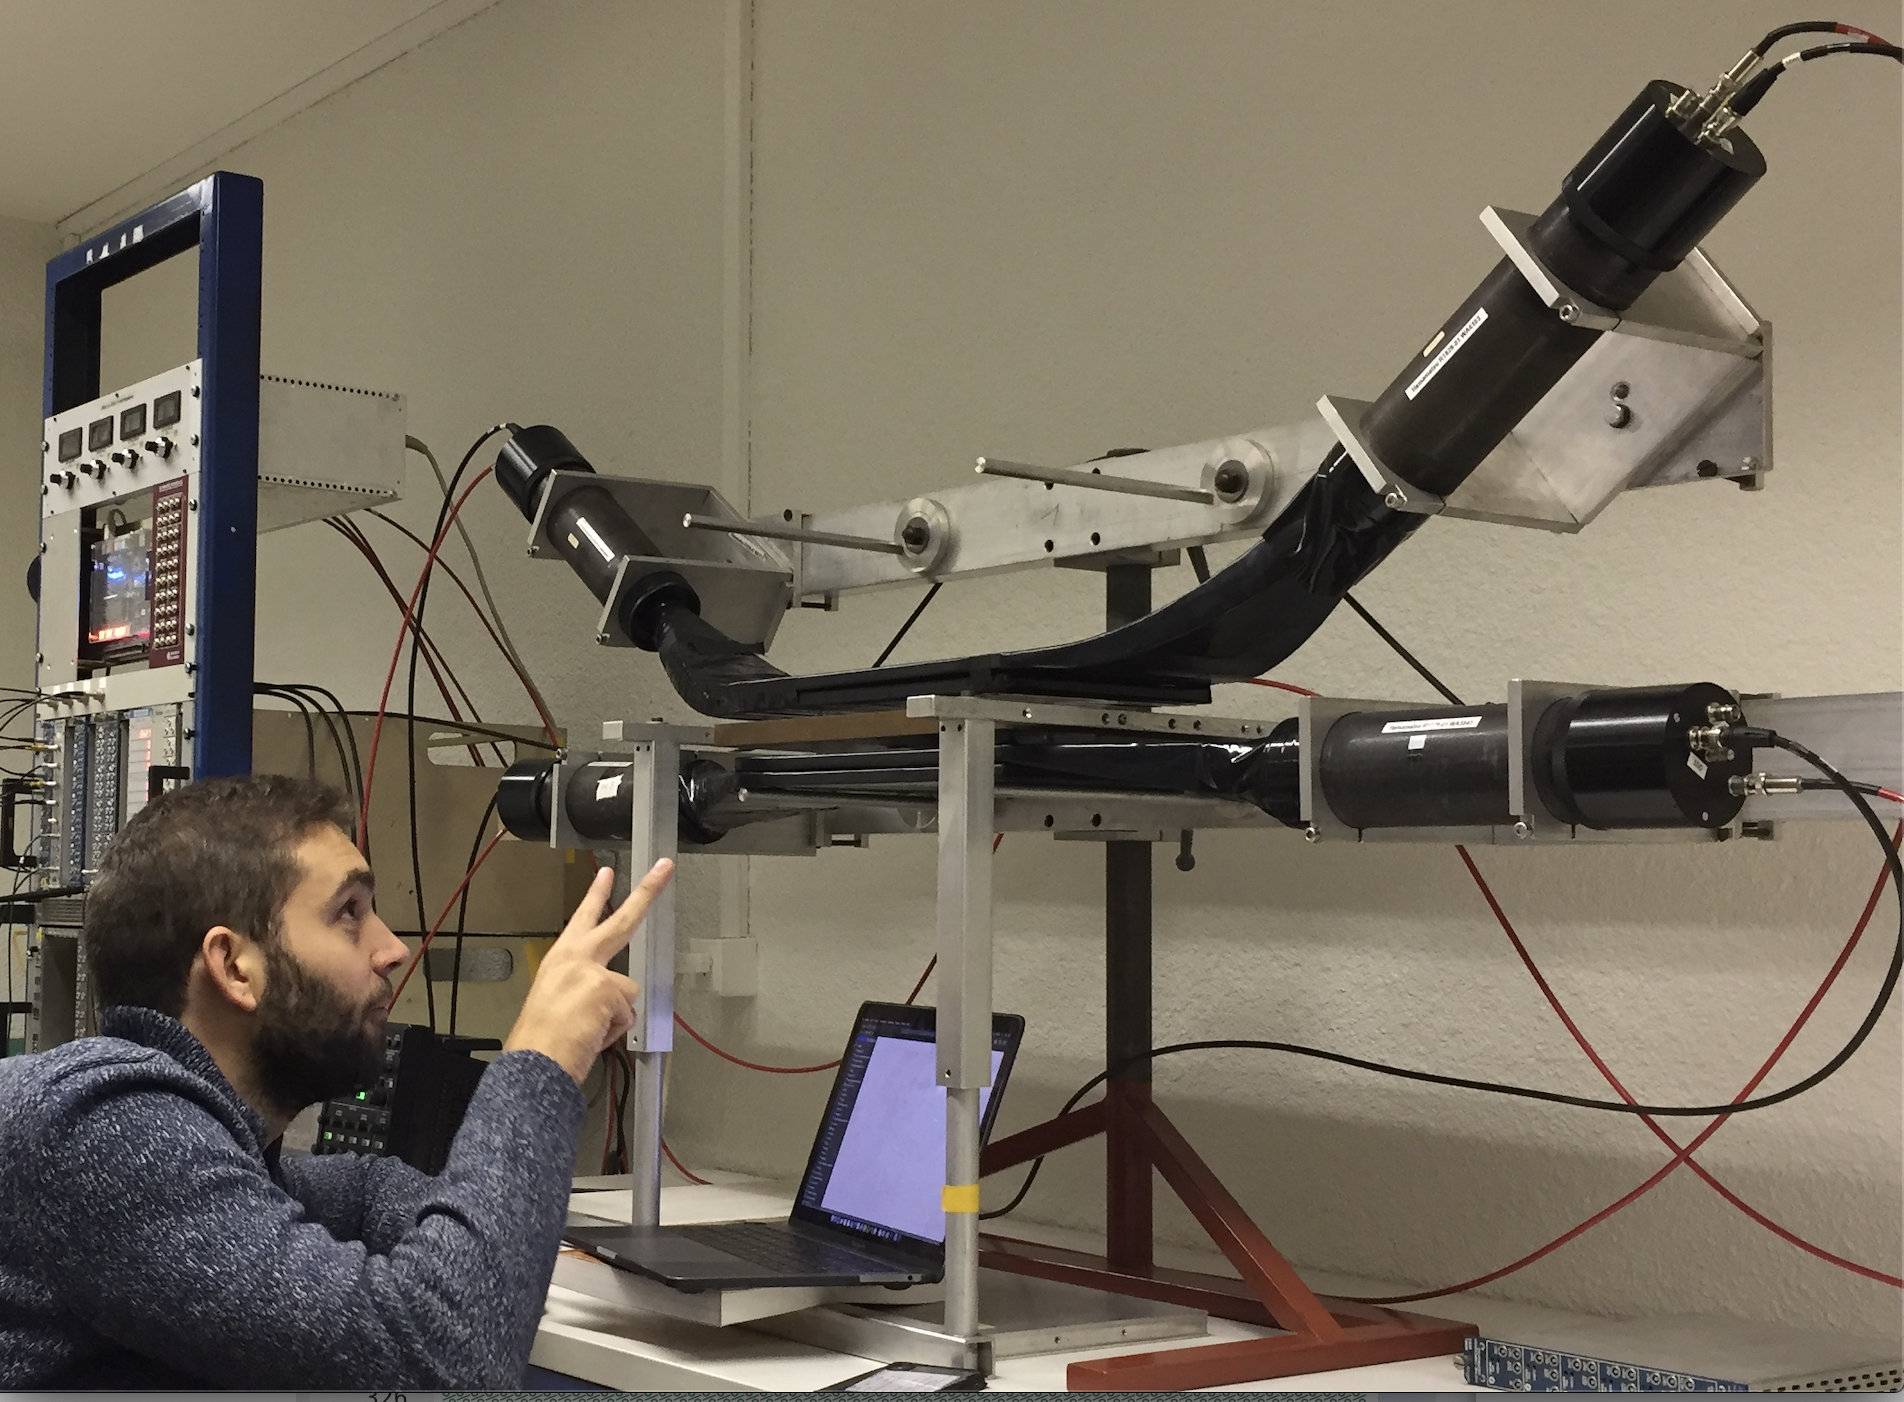
\includegraphics[width=0.8\textwidth]{Images/Photos/Descriptif_expe_1.png}
    \caption{Photo prise représentative de l'expérience. Les divers PMs, scintillateurs }
    \label{fig:Experience_1_montage}
\end{figure}

Le fonctionnement est simple, les particules chargées provenant de l'espace traversent les scintillateurs ainsi que la plaque de métal. Les muons, sont arrêtées par la plaque avant de se désintégrer. Un positron (ou électron dépendant de la charge du muon incident) est alors émis dans une direction (haut ou bas) et sera détecté par un des deux scintillateurs (Up ou Down). Les positrons excitent les molécules du scintillateur qui eu à leurs tours veulent retrouver un état fondamental en émettant des photons et permet la détection.  Ces photons vont alors être dirigés par les guides de lumières vers les PMs (voir les noires présentées sur la Fig. \ref{fig:Experience_1_montage}).

Un photon incident arrive en contacte avec la photo-cathode et y arrache un électron par effet photoélectrique. C'est alors que sous une différence de potentiel entre chaque dynode, cet électron libre va être multiplié afin d'obtenir un signal suffisamment important pour être lisible sur l'oscilloscope (voir Fig. \ref{fig:PM}).

\begin{figure}[htpb!]
    \centering
    \includegraphics[width=0.7\textwidth]{Images/Photos/PM.png}
    \captionsetup{width=0.9\textwidth}
    \caption{Processus de multiplication de l'électron incident à l'intérieur du PM.}
    \label{fig:PM}
\end{figure}

\newpage
%%%%%%%%%%%%%%%%%%%%%%%%%%%%%%%%%%%%%%%%%%%%%%%%%%%%%%%%%%%%%%%%%%%%%%%%%%%%%%%
%%% Code et logiciel quartus labview %%%%%%%%%%%%%%%%%%%%%%%%%%%%%%%%%%%%%%%%%%
%%%%%%%%%%%%%%%%%%%%%%%%%%%%%%%%%%%%%%%%%%%%%%%%%%%%%%%%%%%%%%%%%%%%%%%%%%%%%%%
\subsection{Logiciel de programmation visuel: QUARTUS}

Les signaux sont lu et analysé par QUARTUS, un logiciel en programmation visuel qui permettra de calculer le temps de désintégration des muons de façon automatique.

Les portes logiques que nous avons utilisés sont:
\begin{itemize}
    \item \textbf{And gate}: Si et seulement si les inputs A=B=1 alors la sortie C=1.
    \item \textbf{Or gate}: Si A=1 ou B=1 alors C=1.
    \item \textbf{Not gate}: Elle inverse le signal.
    \item \textbf{Flip-Flop}: Il se comporte comme un interrupteur. Au démarrage du programme la sortie est nul. Si le flip-flop reçoit un signal d'entrée, alors il bascule et sort constamment 1. La seul façon de le remettre à zéro est de lui envoyer un signal sur l'entrée Reset.
    \item \textbf{Horloge}: Elle envoie un signal tout les 20 ns.
    \item \textbf{Compteur}: Il compte le nombre de signal que l'horloge produit.
\end{itemize}

En résumé, notre code commence avec quatre signaux d'entrée correspondant aux quatre signaux des PMs sur la gauche de la Fig. \ref{fig:Quartus}. Ensuite, on veut que si un muon traverse les deux premiers PM du haut (PM1 et PM2) alors on commence à compter le nombre de secondes. Ensuite, une fois que le muon s'est désintégré il y a trois possibilités. Soit le muon sort pas le haut, soit par le bas, soit il n'est pas détecté par les PM et il y aura donc un timeout. Dans ces trois cas on arrête de compter le temps et on exporte les données.
\paragraph{Evenement Start:}
Les quatres signaux des PMs sont numéroté de 1 à 4. PM1 correspond au photomultiplicateur le plus haut et PM4 au plus bas. Nous sommes uniquement intéressé aux particules qui arrivent de l'atmosphère, c'est à dire à ceux qui arrivent du haut. Ainsi, pour déclencher un event start, il faut qu'il y aie une coïncidence sur les PM1 et PM2 et aucun signal sur les PM3 et PM4. Cette condition est atteinte grâce à une porte Not sur PM3 et PM4 et une porte And sur PM1 et PM2. Une fois qu'on sait que un muon à excité les PM1 et PM2 on fait basculer le flip-flop relié au compteur ce qui vas commencé à compter le temps. Il y a de plus un second flip-flop connecté à l'event start de façon à ne pas accidentellement déclenché un "faux start" si les produit de la désintégration du muons sortent par le haut.
\paragraph{Désintégration:}
Une fois que le muon s'est arrêté dans la plaque de matière, il vas se désintégrer et ses constituants vont ressortir dans une direction aléatoire. On veut donc arrêter le chronomètre une fois qu'on détecte les constituants qui ressortent. Il y a trois cas spécifiques à prendre en compte. Le premier cas, est quand les produits du muons sortent par le haut. Ceci provoque alors un signal dans les PM du haut qui vas activer une porte AND (qui n'étaient pas active avant car il faut qu'elle reçoivent aussi un signal que le compteur compte). Cette porte vas arrêter le chronomètre et exporter le temps. Le deuxième cas, est quand les produits sortent par le bas. Alors, le cheminement est similaire à celui d'avant. Le troisième cas, est quand les constituant sortent par un angle non couvert par les PM et donc qui ne sont ni détecté par le haut, ni par le bas. Il faut alors dire au chronomètre de s'arrêter après un certains nombre de bits (qui correspond à un timeout).

\begin{figure}[!ht]
    \centering
    \includegraphics[width=1\textwidth]{Images/Schemas/Quartus.jpg}
    \caption{Code visuel programmé avec QUARTUS permettant de mesurer le temps de vie du muon.}
    \label{fig:Quartus}
\end{figure}

%%%%%%%%%%%%%%%%%%%%%%%%%%%%%%%%%%%%%%%%%%%%%%%%%%%%%%%%%%%%%%%%%%%%%%%%%%%%%%%
%%% Analyse et graphe : Intro %%%%%%%%%%%%%%%%%%%%%%%%%%%%%%%%%%%%%%%%%%%%%%%%%
%%%%%%%%%%%%%%%%%%%%%%%%%%%%%%%%%%%%%%%%%%%%%%%%%%%%%%%%%%%%%%%%%%%%%%%%%%%%%%%
\subsection{Analyse}

Ce chapitre est divisé en deux parties, la première illustre la calibration et la deuxième met en avant les résultats obtenus pour l'étude du Cuivre et pour l'Aluminium.
L'aluminium à comme densité 2.7 $g/cm^{3}$ et le cuivre de 8,96 $g/cm^{3}$. Il en va de soit que le cuivre, ayant une densité plus élevée, est un candidat favorable à de meilleurs résultats. Ceci est du au faite que plus on à de matière plus de chance on aura d'obtenir des interactions entre muons et atomes et donc plus de données seront collectées. 

%%%%%%%%%%%%%%%%%%%%%%%%%%%%%%%%%%%%%%%%%%%%%%%%%%%%%%%%%%%%%%%%%%%%%%%%%%%%%%%
%%% Analyse et graphe : Calibration %%%%%%%%%%%%%%%%%%%%%%%%%%%%%%%%%%%%%%%%%%%
%%%%%%%%%%%%%%%%%%%%%%%%%%%%%%%%%%%%%%%%%%%%%%%%%%%%%%%%%%%%%%%%%%%%%%%%%%%%%%%
\subsubsection{Calibration: expérience temps de vie du Muon}

La première étape consistait à calibrer nos PMs. La manipulation est relativement simple, il suffit de compter le nombre d'évènements obtenus pour un PM et de le diviser par le nombre total d'évènements coïncidant les trois autres PM. En augmentant la tension par paliers, il est facile d'en ressortir un graphique de $\frac{N}{N_{tot}}(U)$. Les résultats obtenus peuvent être observés sur la Fig. \ref{fig:Graph_calib_exp_1}. Sur ce même graphique, des courbes de régression linéaires ont été réalisées et leurs intersections nous définira la tension idéal à prendre pour la suite de l'expérience. La manipulation est à réaliser pour chaque PMs.

\begin{figure}[htpb!]
    \centering
    \includegraphics[width=\textwidth]{graphiques/experience1/calibration/calibration_exp1.png}
    \caption{Calibration des quatres PMs. Les intersections des lignes de régression représentent les tensions optimales à exercer sur chaques PMs. Les valeurs précises sont illustrés dans l'encadré. Par exemple, nous avons reglé le PM3 sur 2300 V.}
    \label{fig:Graph_calib_exp_1}
\end{figure}

\newpage
%%%%%%%%%%%%%%%%%%%%%%%%%%%%%%%%%%%%%%%%%%%%%%%%%%%%%%%%%%%%%%%%%%%%%%%%%%%%%%%
%%% Analyse et graphe : Temps de vie du muon : Cuivre %%%%%%%%%%%%%%%%%%%%%%%%%
%%%%%%%%%%%%%%%%%%%%%%%%%%%%%%%%%%%%%%%%%%%%%%%%%%%%%%%%%%%%%%%%%%%%%%%%%%%%%%%
\subsubsection{Temps de vie du muon : Cuivre}

Dans un premier temps nous avons décidé de travailler séparément avec les données obtenues des deux PMs du dessus ainsi que ceux du dessous. Les résultats peuvent être observés sur la Fig. \ref{fig:comptage_cuivre_up_down_separement}. On voit qu'il y a plus d'évenement sur les PMs du haut comme prédit par la théorie sur l'hélicité.

\begin{figure}[htpb!]
    \centering
    \includegraphics[width=0.8\textwidth]{graphiques/experience1/cuivre/comptage_cuivre_up_down_separement.png}
    \caption{Histogramme en fonction du temps pour les PM up et PM down et pour le cuivre. Ce graphique nous présente le comptage obtenus par les PMs du dessus (en jaune) et du dessous séparément (en bleu). Nous pouvons constater que le taux est de 15\% plus élevé pour la coïncidence du dessus comme prédit par la théorie sur le spin.}
    \label{fig:comptage_cuivre_up_down_separement}
\end{figure}

Il est intéressant de faire un graphique comprenant la totalité des comptages. Celui-ci est présenté sur la Fig. \ref{fig:comptage_total_cuivre}.

\begin{figure}[htpb!]
    \centering
    \includegraphics[width=\textwidth]{graphiques/experience1/cuivre/comptage_total_cuivre.png}
    \caption{Histogramme en fonction du temps de désintégration pour la plaque de cuivre avec coïncidence sur les quatre PMs. L'histogramme suit une décroissance exponentielle.}
    \label{fig:comptage_total_cuivre}
\end{figure}

Une régression exponentielle à été appliquée sur l'histogramme de la Fig. \ref{fig:comptage_total_cuivre}. Les résultats du fit de type $f(x) = e^{(\text{Constante}+\text{Pente}\cdot x)}+\text{Bruit}$ sont:
    \begin{itemize}
        \item \textbf{Constante}: 8.35 $\pm$ $1.19\times10^{-2}$
        \item \textbf{Pente}: $-4.62\times10^{-1}$ $\pm$ $3.9\times10^{-3}$
        \item \textbf{Bruit}: 8.66 $\pm$ $7.61\times10^{-1}$
    \end{itemize}
    
Pour rappel la décroissance des Muons est de type $N(t) = N_{0}\cdot e^{-t/\tau}$. Avec:
    \begin{itemize}
        \item $N_{0}$ = exp(8.35) = $4.24\times10^{3}$ $\pm$ 1.01
        \item $\tau=\frac{1}{0.462} = 2.17 \pm 1.82\times10^{-2}$ \SIUnitSymbolMicro s
    \end{itemize}

La valeur expérimentale obtenue pour le temps de vie du muon est donc de $\tau$ = 2.17 \SIUnitSymbolMicro s ce qui est comparable, en ordre de grandeur, à la valeur du PDG qui était de $\tau$= 2.20 \SIUnitSymbolMicro s ce qui correspond à un écart relatif de seulement 1.4\%.

Plusieurs observations peuvent être faites. La première, est de voir que l'ordre de grandeur entre la valeur pratique et théorique est identique et est de l'ordre du \SIUnitSymbolMicro s. La deuxième constatation qui peut être faite est au sujet des valeurs obtenues. En effet, il est facile d'observer que les deux valeurs sont très proches (2.17 contre 2.20) toutefois en prenant en considération l'erreur obtenue nous n'englobons pas la valeur du PDG. (Car $2.165+0.018=2.182$). Toutefois la valeur est très proche et donc bonne à prendre. Cette différence peut venir de plusieurs facteurs tels que les manipulations, le temps d'exposition ( il aurait peut-être fallu prendre plus de données et ceci sur une plus longue période d'exposition) mais aussi l'état du matériel, en particulier la vieillesse d'un des PM pourrait expliquer cet écart avec le PDG. Pour obtenir un résultat plus rapproché il aurait fallu être plus minutieux. 

Une autre chose que nous avons essayé est de faire un fit, voir la Fig. \ref{fig:UpDownPositifMuonCuivre}, sur uniquement les PMs du haut et du bas. Nous trouvons alors temps de vie pour les muons Up
$\tau_{+\text{Up}}=2.13$ \SIUnitSymbolMicro s et pour les muon  Down $\tau_{+\text{Down}}=2.46$ \SIUnitSymbolMicro s et pour les muons négatif on trouve $\tau_{-\text{Up}}=1.90$ \SIUnitSymbolMicro s et $\tau_{-\text{Down}}=0.732$ \SIUnitSymbolMicro s. Nous avons fait les mesures pour l'aluminium et un recapitulatif des mesures peut être trouvé sur la Table \ref{TauPositifNegatifComplet}.

\begin{figure}[htpb!]
    \centering
    \includegraphics[width=1.0\textwidth]{Images/Photos/UpDownPositifMuonCuivre.jpeg}
    \caption{Fit pour voir la différence entre les PM Up et Down dans le cuivre pour les muons positifs. $\tau_{+\text{Up}}=2.16$ \SIUnitSymbolMicro s et $\tau_{+\text{Down}}=2.26$ \SIUnitSymbolMicro s }
    \label{fig:UpDownPositifMuonCuivre}
\end{figure}

\begin{figure}[htpb!]
    \centering
    \includegraphics[width=1.0\textwidth]{Images/Photos/UpDownNegatifMuonCuivre.jpeg}
    \caption{Fit pour voir la différence entre les PMs Up et Down dans le cuivre pour les muons négatif. $\tau_{-\text{Up}}=1.90$ \SIUnitSymbolMicro s et $\tau_{-\text{Down}}=0.732$ \SIUnitSymbolMicro s}
    \label{fig:UpDownNegatifMuonCuivre}
\end{figure}

\begin{figure}[htpb!]
    \centering
    \includegraphics[width=1.0\textwidth]{Images/Photos/UpDownPositifMuonAlu.jpeg}
    \caption{Fit pour voir la différence entre les PM Up et Down dans l'aluminium pour les muons positifs. $\tau_{+\text{Up}}=2.08$ \SIUnitSymbolMicro s et $\tau_{+\text{Down}}=2.13$ \SIUnitSymbolMicro s }
    \label{fig:UpDownPositifMuonAlu}
\end{figure}

\begin{figure}[htpb!]
    \centering
    \includegraphics[width=1.0\textwidth]{Images/Photos/UpDownNegatifMuonAlu.jpeg}
    \caption{Fit pour voir la différence entre les PMs Up et Down dans l'aluminium pour les muons négatif. $\tau_{-\text{Up}}=1.32$ \SIUnitSymbolMicro s et $\tau_{-\text{Down}}=0.537$ \SIUnitSymbolMicro s}
    \label{fig:UpDownNegatifMuonAlu}
\end{figure}

\begin{table}[htbp!]
  \centering
  \captionsetup{width=0.9\textwidth}
  \caption{Résulats expérimentaux pour le temps de vie des muons positifs et négatifs dans les PM up et down.}
  \begin{tabular}{lc|cccc}
     & & $+$ Cuivre  & $+$ Aluminium & $-$ Cuivre & $-$ Aluminium \\
    \hline
    Up &  $\tau$ & 2.16 & 2.08 & 1.90 & 1.32\\
    &Entrées & 13'462 & 11'611 & 13'462 & 11'611 \\
    & $\chi^{2}$ & 1.13 & 0.50 & 1.55 & 1.95\\
    & Prob. & 0.311 & 0.95 & 0.034 & 0.002\\
    \hline
    Down & $\tau$ & 2.26 & 2.13 & 0.732 & 0.537 \\
    &Entrées & 10'402 & 10'964  & 10'402 & 10'964\\
    &$\chi^{2}$ & 0.96 & 0.91 & 1.15 & 1.34 \\
    &Prob. & 0.54 & 0.96 & 0.27 & 0.11\\
    \hline
    Prédiction [5] & & 2.2 & 2.2 & 0.16 & 0.88 \\
    
\end{tabular}
\label{TauPositifNegatifComplet}
\end{table}

%%%%%%%%%%%%%%%%%%%%%%%%%%%%%%%%%%%%%%%%%%%%%%%%%%%%%%%%%%%%%%%%%%%%%%%%%%%%%%%
%%% Analyse et graphe : Temps de vie du muon : Cuivre %%%%%%%%%%%%%%%%%%%%%%%%%
%%%%%%%%%%%%%%%%%%%%%%%%%%%%%%%%%%%%%%%%%%%%%%%%%%%%%%%%%%%%%%%%%%%%%%%%%%%%%%%
\newpage
\subsubsection{Oscillation journalière du flux muonique : Cuivre}

Une deuxième thématique abordée durant ce travail pratique à été la variation du flux muonique en fonction de l'heure dans une journée. Nous cherchons à déterminer si l'origine du flux muonique est solaire ou est de provenance cosmique. Si les muons sont crée par le soleil, alors,une variation jour-nuit pourrait être observée. 
La terre étant très proche du soleil, celui-ci pourrait être la principale source de muons détectés sur la terre et l'isotropie cosmologique (c'est-à-dire qu'il n'existe pas de direction privilégiée pour une observation) pourait être écartée.
Nous savons que par exemple un muon de 1 GeV parcourra en moyenne 6 km dans l'atmosphère et qu'un muon de 10 GeV parcourra près de 63 km. De plus, en pleine nuit, le soleil étant de l'autre coté de la terre, uniquement les muons de hautes énergies pourront traverser la terre et donc être détectés par notre expérience. Une diminution du flux muonique est donc prévisible durant la nuit. Nous avons essayé de démontrer cela en ajoutant dans notre code Quartus un prise de l'heure, des minutes et  des secondes à laquelle un évènement à été collecté et nous avons pu en faire un histogramme. Le nombre d'évènements total collectés pour cette mesure étaient de 13462. La Fig. \ref{fig:oscillation_jour_cuivre} nous présente ces résultats avec la partie du dessus représente les évènements obtenus par coïncidence des deux PMs du dessus alors que le graphique du dessous présente les résultats obtenus par coïncidence des PMs du dessous. L'axe des abscisses va 0 à 1440 minutes représentant le nombre de minutes en une journée ($24\cdot60=1440$) et l'axe des ordonnées représente le comptage par minute. La Fig. \ref{fig:oscillation_jour_cuivre_total} illustre les résultats accumulés sur une semaine. Les deux figures montrent qu'il y à bien des oscillations du flux mais les régressions sinusoïdale appliquée sur les données ne sont pas synchronisées avec le cycle jour/nuit et celles-ci sont juste du bruit.  Nous pouvons donc en conclure qu'il n'y a pas changement mesurable de flux cosmique entre le jour et la nuit (ils ne sont pas crée par le soleil). Les muons sont de nature cosmique avec une direction isotrope.

\begin{figure}[htpb!]
    \centering
    \includegraphics[width=0.8\textwidth]{graphiques/experience1/cuivre/OSCILLATION_JOUR_CUIVRE.png}
    \caption{Résultats du comptage pour la plaque de cuivre en fonction de l'heure en une journée. On n'observe pas de fluctuation jour/nuit.}
    \label{fig:oscillation_jour_cuivre}
\end{figure}

\begin{figure}[htpb!]
    \centering
    \includegraphics[width=0.8\textwidth]{graphiques/experience1/cuivre/oscillation_jour_cuivre_total_comptage.png}
    \caption{Résultats du comptage pour la plaque de cuivre en fonction de l'heure en une journée. Données prises sur une semaine. Nous n'observons pas de correlation avec le soleil.}
    \label{fig:oscillation_jour_cuivre_total}
\end{figure}


\newpage
%%%%%%%%%%%%%%%%%%%%%%%%%%%%%%%%%%%%%%%%%%%%%%%%%%%%%%%%%%%%%%%%%%%%%%%%%%%%%%%
%%% Analyse et graphe : Temps de vie du muon : Aluminium %%%%%%%%%%%%%%%%%%%%%%
%%%%%%%%%%%%%%%%%%%%%%%%%%%%%%%%%%%%%%%%%%%%%%%%%%%%%%%%%%%%%%%%%%%%%%%%%%%%%%%
\subsubsection{Temps de vie du muon : Aluminium}

La même expérience à été reproduite avec une plaque d'aluminium et les résultats du fit de type $f(x) = e^{(\text{Constante}+\text{Pente}\cdot x)}+\text{Bruit}$ sont: 

\begin{itemize}
    \item \textbf{Constante}: 8.41 $\pm$ $1.29\times10^{-2}$
    \item \textbf{Pente}: $-5.08\times10^{-1}$ $\pm$ $4.60\times10^{-3}$
    \item \textbf{Bruit}: 6.99 $\pm$ $5.83\times10^{-1}$
\end{itemize}
    
Pour rappel la décroissance Muon est de type $N(t) = N_{0}\cdot e^{-t/\tau}$
\begin{itemize}
    \item $N_{0}$ = $e^{8.41}$ = $4.47\times10^{3}$ $\pm$ 1.01
    \item $\tau=\frac{1}{0.508}$ = 1.97 $\pm$ $4.31\times10^{-1}$ \SIUnitSymbolMicro s
\end{itemize}


La Fig. \ref{fig:comptage_Aluminium_up_down_separement} nous présente le détaillé des coïncidences up and down avec une plaque d'aluminium alors que la Fig. \ref{fig:comptage_total_aluminium} nous présente le comptage total.


\begin{figure}
    \centering
    \includegraphics[width=0.8\textwidth]{graphiques/experience1/Aluminium/comptage_Aluminium_up_down_separement.png}
    \caption{Résultats Comptage PM up et PM down pour l'aluminium. Ce graphique nous présente le comptage obtenus par les PMs du dessus (en jaune) et du dessous séparément (en bleu). Nous pouvons constater que le taux est à nouveau plus élevé pour la coïncidence du dessus}
    \label{fig:comptage_Aluminium_up_down_separement}
\end{figure}

\begin{figure}
    \centering
    \includegraphics[width=0.8\textwidth]{graphiques/experience1/Aluminium/comptage_total_Aluminium.png}
    \caption{Histogramme en fonction du temps pour la plaque d'aluminium. L’histogramme suit une décroissance exponentielle. La ligne rouge représente la régression exponentielle.}
    \label{fig:comptage_total_aluminium}
\end{figure}

Les Fig. \ref{fig:comptage_total_aluminium} et \ref{fig:comptage_Aluminium_up_down_separement} suivent la même décroissance exponentielle que celle présentée sur les Fig. \ref{fig:comptage_total_cuivre} et \ref{fig:comptage_cuivre_up_down_separement}. Ceci nous confirme donc l'éligibilité des résultats obtenus aussi bien pour la manipulation avec la plaque de cuivre que celle avec la plaque d'aluminium. Nous noterons quand même que les résultats obtenus lors de cette deuxième manipulation sont moins précis. En effet la valeur du temps de vie obtenu est de $\tau=1.97$ $\pm$ $4.31\times10^{-1}$ \SIUnitSymbolMicro s. Alors que la valeur du PDG est de $\tau=2.20$ \SIUnitSymbolMicro s ce qui correspond à un écart relatif de 10.3\%. Néanmoins nous pouvons voir que la valeur obtenue englobe la valeur du PDG si on prend en compte les erreurs ce qui est bon signe. 

\subsubsection{Détermination du temps de vie des muons positif et négatif}

Pour extraire les temps de vie des muons positif $\tau^{+}_{\mu}$ et négatif $\tau^{-}_{\mu}$ nous utilisons la méthode proposé dans la théorie. Nous faisons d'abord une régression exponentielle sur une région sans muons négatif puis nous réinjectons les valeurs du fit sur l'ensemble des mesures et nous obtenons les résultats de la Table \ref{TauPositifNegatif}:


\begin{table}[htbp!]
  \centering
  \captionsetup{width=0.9\textwidth}
  \caption{Résulats expérimentaux pour le temps de vie des muons positifs et négatifs.}
  \begin{tabular}{cccccc}
     Valeur & N$^{\text{o}}$ Entrées & Expérimentale & $\chi^{2}/ndf$  & Théorique & $\epsilon$ \%\\
    \hline
    Cuivre $\tau_{+}$ & 23684 & 2.26 & 0.94 & 2.20 & 2.7\\
    Cuivre $\tau_{-}$ & 23684 & 0.24 & 1.53 & 0.16 & 50 \\
    Alu $\tau_{+}$ & 22575 & 2.16 & 0.68 & 2.20 & 1.8\\
    Alu $\tau_{-}$ & 22575 & 0.68 & 1.07 & 0.88 & 22\\
\end{tabular}
\label{TauPositifNegatif}
\end{table}

\begin{landscape}
\begin{figure}[htbp!] 
\centering  
    \begin{subfigure}[t]{.7\textwidth}
    \includegraphics[width=.9\textwidth]{Images/Photos/TauPlusCuivre.jpeg}
    \captionsetup{width=0.8\textwidth}
    \caption{Fit sur le temps de vie avec plaque en cuivre pour déterminer la temps de vie des muons positif. La région sans muon négatif a été sélectionée. Nous obtenons $\tau_{+}=2.26$ \SIUnitSymbolMicro s.}
    \label{fig:TauPlusCuivre}
    \end{subfigure}
    \begin{subfigure}[t]{.7\textwidth}
    \includegraphics[width=.9\textwidth]{Images/Photos/TauMoinsCuivre.jpeg}
    \captionsetup{width=0.8\textwidth}
    \caption{Fit sur le temps de vie avec plaque en cuivre pour déterminer la temps de vie des muons négatif. Nous obtenons $\tau_{-}=0.24$ \SIUnitSymbolMicro s.}
    \label{fig:TauMoinsCuivre}
    \end{subfigure}
    \begin{subfigure}[t]{.7\textwidth}
    \includegraphics[width=0.9\textwidth]{Images/Photos/TauPlusAlu.jpeg}
    \captionsetup{width=0.8\textwidth}
    \caption{Fit sur le temps de vie avec plaque en Alu pour déterminer la temps de vie des muons positif. Nous obtenons $\tau_{+}=2.16$ \SIUnitSymbolMicro s.}
    \label{fig:TauPlusAlu}
    \end{subfigure}
    \begin{subfigure}[t]{.7\textwidth}
    \includegraphics[width=.9\textwidth]{Images/Photos/TauMoinsAlu.jpeg}
    \captionsetup{width=0.8\textwidth}
    \caption{Fit sur le temps de vie avec plaque en Alu pour déterminer la temps de vie des muons négatif. Nous obtenons $\tau_{-}=0.68$ \SIUnitSymbolMicro s.}
    \label{fig:TauMoinsAlu}
    \end{subfigure}
\caption{Détermination des temps de vie pour les muons positif et négatif.}
\label{TempsDeVieMuonPositifNegatif}
\end{figure}
\end{landscape}

%%%%%%%%%%%%%%%%%%%%%%%%%%%%%%%%%%%%%%%%%%%%%%%%%%%%%%%%%%%%%%%%%%%%%%%%%%%%%%%
%%% Analyse et graphe : Synthèses des résultats %%%%%%%%%%%%%%%%%%%%%%%%%%%%%%%
%%%%%%%%%%%%%%%%%%%%%%%%%%%%%%%%%%%%%%%%%%%%%%%%%%%%%%%%%%%%%%%%%%%%%%%%%%%%%%%
\subsection{Synthèse des résultats}

Lors de cette expérience nous avons calculé le temps de vie des muons et ceci par l'intermédiaire de leurs désintégrations dans deux matériaux. En voici les résultats obtenus: 

\begin{center}
 \begin{tabular}{ll} 
 Matériel & $\tau$ \SIUnitSymbolMicro s \\
 \hline
 Cuivre & 2.17 $\pm$ $1.828\times10^{-2}$ \\ 
 Aluminium & 1.97 $\pm$ $4.31\times10^{-1}$ \\
  PDG & 2.20 $\pm 2.2\times10^{-6}$ \\
\end{tabular}
\end{center}

Les résultats obtenus ont un ordre de grandeur similaire à la valeur théorique du PDG ce qui confirme leur cohérence. Néanmoins, comme expliqué dans les paragraphes précédant, les valeurs sont certes proche de celle du PDG mais diffèrent quand même. Plusieurs sources d'erreurs peuvent être prises en considérations: 

\begin{itemize}
    \item La superficie de l'expérience: La surface des scintillateurs est de 600 $cm^{2}$. Avec une aussi petite surface, et sachant que le passage d'un muon est un processus stochastique, nous pouvons avoir ou pas de la chance et donc avoir une situation favorable ou non à la détection des muons. Avoir une surface plus grande serait idéal pour augmenter la chance d'obtenir un nombre plus élevé de muons traversant notre plaques. 
    
    \item Orientation des détecteurs: Si nous partons du principe que nous sommes très proche du soleil, et donc que celui-ci est la principale source de muons alors il faudrait que l'expérience suive de façon dynamique le soleil (avec un moteur par exemple). La situation idéale serait d'avoir le flux de muons arrivant perpendiculairement à notre expérience.
    
    \item Les obstacles au dessus de l'expérience: comme toutes particules voyageant, les muons interagissent avec la matière. C'est pourquoi, être dans un sous-sol, avec un bâtiment de plusieurs étages au dessus réduit drastiquement le nombre de muons pouvant arriver et donc se désintégrer dans nos scintillateurs. La situation idéale serait d'être sur le toit de l'école de physique.
    
\end{itemize}

Dans un deuxième temps, il est intéressant de s'attarder un moment sur le flux des muons obtenus. En effet, nous savons que de manière générale au niveau de la mer, le flux de muons est d’environ 170 muons par m$^{2}$ et par seconde \cite{noauthor_radioactivite_nodate}, si bien que nous sommes traversés par une trentaine de muons par seconde. Regardons ce que nous avons obtenus: 

\begin{center}
\begin{tabular}{lrrrc}
     Matériel & Secondes & Jours & N$^{\text{o}}$ Muons & N$^{\text{o}}$ Muon par s$\cdot$m$^2$\\
     \hline
     Cuivre &  1824004 & 21,1 & 23864 & 0.218 \\
     Aluminium & 1807179 & 20,9 & 22575 & 0.209 \\
\end{tabular}
\end{center}

Le flux moyen de muons interagissant est de l'ordre de $(0.218+0.209)/2=0.2135$. Ceci représente à peine le 1.4\% de ce que nous devrions obtenir (à savoir les 170 muons par m$^2$ et par secondes, dans le cas de notre expérience faisant 600 cm$^{2}$, ceci équivaut à $10'000$ cm$^{2}/600$ cm$^{2}=16.667$ et donc, un facteur de 17 de moins. Nous devrions alors trouver $170/17=10$ muons$\cdot$ s$^{-1}\cdot $m$^{-2}$ . Dans un cas idéal, sans toit, au niveau de la mer et bien entendu avec un dispositif optimal, nous devrions atteindre les 10 muons par secondes avec notre expérience. Ceci avec un régime stochastique favorable et moyenné sur une longue période de prise de mesure. Plusieurs causes peuvent amener à cette différence: 

\begin{itemize}
    \item La qualité du matériel utilisé: Le matériel étant vieux, le rendement à sans doutes diminué depuis la première utilisation. D'ailleurs nous avions eu des soucis avec un PM. Ceci est relativement bien visible sur la Fig. \ref{fig:Graph_calib_exp_1} ou le PM D est moins performant que les trois autres. C'est pourquoi nous avons du monter plus haut en Tension afin d'atteindre le pallier de calibration. Ce genre de manipulation n'est pas sans risques car une tension trop élevée peut générer plus de bruit mais aussi affaiblir d'avantage l'électronique à l'intérieur en grillant les circuit électrique.
    
    \item L'énergie transportée par les muons: Nous savons que les muons voyageant peuvent transporter une quantité différente d'énergie au cours de leurs voyage. Bien entendu seuls les muons possédant une quantité d'énergie relativement faible interagissaient avec notre expérience. Une proportion du flux muonique est alors freiné et se désintègre au contact de nos plexiglas. Cependant une autre proportion, possédant une énergie plus importante passe sans ioniser le milieu absorbeur. Cette proportion est donc une des causes du manque cité au-dessus.
    
    \item La direction des photons émis après interaction: Le photon émis après interaction du muon est complètement aléatoire c'est pourquoi si celui-ci est émis horizontalement, ce photon atteindra plus rapidement le PM. Son temps de dérive sera alors plus court. 
    
    \item Le temps de travail de la carte Quartus: Le processus à un temps de travail minimum. Deux évènements dont la différence de temps est plus petite que le temps du processeur, le deuxième évènement sera alors perdu.
\end{itemize}

    En outre, il est facile de constater que les nombres de muons obtenus par secondes et par m$^{2}$ sont très similaires entre le cuivre et l'aluminium. Nous avons obtenus 0.218 muons$\cdot$s$^{-1}\cdot$m$^{2}$ pour le cuivre et 0.209 muons$\cdot$s$^{-1}\cdot$m$^{2}$ pour l'aluminium. En effet se sont deux valeurs très proche. Ceci est très intéressant car nous pouvons alors affirmer que la réussite de l'expérience ne dépend pas forcement du type de matériel que nous choisissons (Cuivre, Aluminium, etc...) mais au contraire, que celle-ci, dépend du lieu dans lequel on se trouve pour réaliser l'expérience. Par exemple, faire ce type d'expériences sur le toit de l'université (où se situe le télescope, au dessus de science 2) aurait été plus intéressant. Ceci aurait pu nous amener à des résultats plus précis. 

\begin{comment}
\subsubsection{Relation temps de demie-vie et masse du muon}
Dans le cours de M. Bravar nous avons pu voir que la masse du muon est liée au temps de demie-vie de celui-ci: voir Éq. \ref{equ_time_mass_muon} représentant la désintégration du muon dans nos deux plaque. Cette équation est issue du slide numéro 7, page 10 du cours de PPA2.
\begin{equation}
\Gamma\left(\mu^{+} \rightarrow e^{+} \overline{v}_{\mu} v_{e}\right)=\frac{G_{F}^{2}}{192 \pi^{2}} m_{\mu}^{5} \propto G_{F}^{2}\cdot m_{\mu}^{5} 
\label{equ_time_mass_muon}
\end{equation}
Si la constante de Fermi $G_{F}$ est considérée comme connue et valant $G_{F}=1.16637\pm0.00001\cdot10^{-5} \text{GeV}^{-2}$, nous pouvons alors déduire de nos résultats d'expérience, la valeur de la masse du muon. En voici les résultats obtenus:
\begin{center}
\begin{tabular}{ll}
    Matériel & $m_{\mu}$ MeV\\
    \hline
    Cuivre & 105.9 $\pm$ 1.5 \\
    Aluminium & 107.9 $\pm$ 2.8\\
    PDG & 105.7 $\pm$ 3.8$\times10^{-6}$ \\
\end{tabular}
\end{center}
Les résultats sont approximatifs mais restent proches de la valeur du PDG. Ceci est très intéressant et confirme que l'on peut utiliser notre expérience pour calculer la masse du muon. Cependant nous constatons quand même que la valeur obtenue à une erreur relativement élevée en comparaison avec celle de la valeur du PDG. 
\end{comment}

\subsubsection{Constante de Fermi}
Pour vérifier la valeur de la constante de Fermi $G_{F}$, nous pouvons utiliser la formule suivante:
\[ G_{F} =8\sqrt{\frac{3\pi^{3}}{m_{\mu}^{5}\tau_{\mu}}} \]
où $m_{\mu}=0.105$ GeV est la masse du muon.
Si on utilise la valeur expérimental du cuivre et de l'aluminium du temps de vie du muon $\tau_{\mu}=2.17\times10^{-6} \text{ s}$ et qu'on la convertis en unités naturelle en utilisant que 1 GeV$^{-1}\rightarrow6.58\times10^{-25}$ s on obtient:

\[ \tau_{\mu_{Cuivre}}=3.29\times10^{18}\,\text{GeV}^{-1}\]
\[ \tau_{\mu_{Alu}}=2.99\times10^{18}\,\text{GeV}^{-1}\]

Et on trouve comme valeur pratique pour le Cuivre:

\[ G_{F_{Cuivre}}=1.19\times10^{-5}\,\text{GeV}^{-2}\]
\[ G_{F_{Alu}}=1.25\times10^{-5}\,\text{GeV}^{-2}\]

qui sont des valeurs proche de la valeur du PDG: $G_{F}=1.17\times10^{-5}\,\text{GeV}^{-2}$ avec une erreur relative de  1.7\% pour le cuivre et de 6.8\% pour l'aluminium.


%%%%%%%%%%%%%%%%%%%%%%%%%%%%%%%%%%%%%%%%%%%%%%%%%%%%%%%%%%%%%%%%%%%%%%%%%%%%%%%
%%% Améliorations %%%%%%%%%%%%%%%%%%%%%%%%%%%%%%%%%%%%%%%%%%%%%%%%%%%%%%%%%%%%%
%%%%%%%%%%%%%%%%%%%%%%%%%%%%%%%%%%%%%%%%%%%%%%%%%%%%%%%%%%%%%%%%%%%%%%%%%%%%%%%
\subsection{Améliorations et suggestions}

La première amélioration qui pourrait être faite concernerait le matériel. En effet Comme nous pouvons le constater sur le graphique représentant la calibration de l'expérience (Fig. \ref{fig:Graph_calib_exp_1}), le PM numéro B (celui en bleu) à une ascension retardée en tension. Il faut donc monter plus haut en tension afin d'atteindre le palier. Ce qui est signe d'une possible vieillesse du matériel. Avec l'usure, il se pourrait que dans les prochaines années, ce instrument surchauffe et donc ne soit donc plus utilisable. Il serait conseillé de le changer. 

La deuxième amélioration qui pourrait être faite sur ce laboratoire est la variation du flux de muon sur 24h. Comme nous avons pu le constater, nous avons tenté de le réaliser mais malheureusement le nombre de données prises n'était pas suffisant. Il aurait fallu prendre sur une période plus longue. Les résultats obtenus sont présenté sur la Fig. \ref{fig:oscillation_jour_cuivre} pour le cuivre. Nous n'avons malheureusement pas eu le temps de procéder à la manipulation pour l'aluminium ou sur des autres matériaux. Il serait intéressant de refaire la manipulation afin de voir si le flux varie en fonction de la journée, dans ce cas la, le soleil serait donc un apport muonique non négligeable ce qui signifierait que le soleil serait la plus grande source de muons dans le voisinage de la terre. Ce qui signifierait que la majorité des muons détectés sur terre seraient crées par le soleil.

Dans le cas inverse ou la variation de muon serait moindre alors ceci permettrait de confirmer la théorie mettant en avant la propriété isotropique de l'espace. Et alors dans ce cas le soleil ne jouerait pas un grand rôle dans la création des muons détectés sur terre. Bien entendu ceci est une proposition d'expérience, il faudrait voir si l'expérience que nous avons utilisées permet de répondre à cette question...

%%%%%%%%%%%%%%%%%%%%%%%%%%%%%%%%%%%%%%%%%%%%%%%%%%%%%%%%%%%%%%%%%%%%%%%%%%%%%%%
%%% Conclusion locale  %%%%%%%%%%%%%%%%%%%%%%%%%%%%%%%%%%%%%%%%%%%%%%%%%%%%%%%%
%%%%%%%%%%%%%%%%%%%%%%%%%%%%%%%%%%%%%%%%%%%%%%%%%%%%%%%%%%%%%%%%%%%%%%%%%%%%%%%
\subsection{Résumé des mesures}

En utilisant une plaque de cuivre et d'aluminium, nous avons obtenus pour le temps de demie-vie du muon les valeurs suivantes: 

\begin{center}
\begin{tabular}{lr}
    Matériel & $\tau$ \SIUnitSymbolMicro s   \\
    \hline
    Cuivre & 2.16492 $\pm$ 0.01828 \\
    Aluminium & 1.96872 $\pm$ 0.4314\\
    PDG &  2.1969811 $\pm $0.0000022 \\
\end{tabular}
\end{center}

On peut constater que les valeurs sont en accord avec valeur issue du PDG ce qui nous laisse à croire que dans son ensemble, l'expérience s'est bien déroulée.


\newpage
%%%%%%%%%%%%%%%%%%%%%%%%%%%%%%%%%%%%%%%%%%%%%%%%%%%%%%%%%%%%%%%%%%%%%%%%%%%%
%%%%%%%%%%%%%%%%%%%%%%%%%%%% DEUXIEME EXPERIENCE%%%%%%%%%%%%%%%%%%%%%%%%%%%%
%%%%%%%%%%%%%%%%%%%%%%%%%%%%%%%%%%%%%%%%%%%%%%%%%%%%%%%%%%%%%%%%%%%%%%%%%%%%
\section{Mesure du flux cosmique}
Durant le deuxième partie de notre laboratoire nous nous sommes intéressés au flux cosmique. Le but était de mettre en place un télescope à muons capable de non seulement les détecter, comme pour l'expérience précédente, mais en plus de pouvoir étudier les muons provenant de toutes les directions dans le ciel. Le dispositif possède deux degrés de libertés suivant les angles azimutale et méridional. Nous allons vous expliquer, pas à pas la manière dont nous avons procédé. 

\subsection{Procédure de construction}
La procédure à été divisée en deux grosses parties: la réalisation des pièces puis le montage. 

\subsubsection{Réalisation de pièces}
Nous avons eu la chance de pouvoir participer à la fabrication de ce télescope à muons en nous occupant de la partie collage et enrobage des quatre scintillateurs. 

\begin{itemize}
    \item \textbf{La fabrication des scintillateurs: } Pour notre part, la fabrication des scintillateurs était restreinte au collage des différentes parties entre elles. À savoir une partie scintillante (qui est divisée en deux parties, une carrée et une autre en forme de cône, cette partie scintillante peut être observée sur la Fig. \ref{fig:Scintillateur}),  une partie en plexiglas (conduisant la lumière, celle-ci est en forme de cylindre) et permettant l'emboîtage avec les photon-multiplicateurs. Une colle sous forme de résine à été utilisée afin de les coller. Celle-ci est choisie pour ce genre de manipulations par sa caractéristique à être fortement perméable à la lumière (ce qui diminue le coefficient de réflexion entre les deux matériaux. Cette étape à été principalement réalisée par Coralie. Notre charge de travaille, chacun, consistait à coller, pour un scintillateur, les deux parties scintillantes (celle carrée et celle de forme conique) entre elles. 
    
\begin{figure}[htbp!] 
\centering  
    \begin{subfigure}[t]{.45\textwidth}
    \includegraphics[width=1.0\textwidth]{Images/Photos/scintilateur.jpg}
    \captionsetup{width=0.8\textwidth}
    \caption{Les scintillateurs sont en trois parties: une forme cylindrique en plexiglas qui conduit la lumière et s'emboîte dans le PM. Une partie en cône pour guider la lumière et un carré scintillant qui produit des photons.}
    \label{fig:Scintillateur}
    \end{subfigure}
    \begin{subfigure}[t]{.45\textwidth}
    \includegraphics[width=1.0\textwidth]{Images/Photos/couche_scintilateur.jpg}
    \captionsetup{width=0.8\textwidth}
    \caption{Enrobage d'un scintillateur par une couche d'aluminium et de plastique noir servant à éviter toute fuite de lumière.}
    \label{fig:couche_scintilateur}
    \end{subfigure}
\caption{Photo des scintillateurs.}
\label{Scintillateurs2Fig}
\end{figure}

    \item \textbf{L'assemblage des PMs: } Pour assembler des photon-multiplicateurs avec les scintillateurs, nous avons utilisé de l'aluminium, des feuilles plastifiées noires imperméable à la lumière ainsi que du scotch noir afin de combler les jonctions. Le but de la manipulation est de recouvrir les scintillateurs avec une première couche d'aluminium, puis avec les feuilles de plastique noir et finalement boucher leurs jonctions avec des bouts de scotch, voir Fig. \ref{fig:couche_scintilateur}. Cette manipulation est cruciale car une seule petite fuite de lumière peut fortement modifier les résultats. Une trou laissant entrer de la lumière augmente considérablement le nombre d'électrons multipliés par nos PM. Des électrons venant de l'extérieur du PM augmenteront alors la tension finale issue du PM. Si la tension introduite est élevé alors celui-ci peut griller. Une photos des photo-multiplicateurs peut être aperçu sur la Fig. \ref{fig:PMS_photo}.
    
    \begin{figure}[htpb!]
        \centering
        \includegraphics[width=0.9\textwidth]{Images/Photos/PM_photo.jpg}
        \caption{Chevauchement des scintillateurs. Une fuite de lumière, augmente considérablement la tension à l'intérieur des PM et un risque de surcharge peut avoir lieu. Il faut faire attention d'avoir bouché tous les trous.}
        \label{fig:PMS_photo}
    \end{figure}

    \item \textbf{Le montage de la structure externe: } Cette partie c'est faite relativement rapidement. Nous avons reçu les pièces séparée et il a fallu les assembler entre elles avec divers boulons et vis. Le rendu final de notre expérience peut être observé sur la figure numéro \ref{fig:Structure_integrale}.
    \begin{figure}[htpb!]
        \centering
        \includegraphics[width=0.7\textwidth]{Images/Photos/Structure_integrale_exp.jpg}
        \caption{Structure intégrale du télescope à muons.}
        \label{fig:Structure_integrale}
    \end{figure}
    
    \end{itemize}


%%%%%%%%%%%%%%%%%%%%%%%%%%%%%%%%%%%%%%%%%%%%%%%%%%%%%%%%%%%%%%%%%
%%% ANALYSE DES DONNEES  %%%%%%%%%%%%%%%%%%%%%%%%%%%%%%%%%%%%%%%%
%%%%%%%%%%%%%%%%%%%%%%%%%%%%%%%%%%%%%%%%%%%%%%%%%%%%%%%%%%%%%%%%%

\subsection{Calibration}

Tous comme pour l'expérience précédente, la première étape consistait à calibrer nos photo-multiplicateurs. Il s'agissait de compter le nombre d'évènements obtenus pour un PM et de le diviser par le nombre total d'évènements coïncidant avec les trois autres photo-multiplicateurs.  Le graphique présenté sur la Fig. \ref{fig:Graph_calib_exp_2} nous présente les résultats obtenus. 
De la même manière que pour la première expérience, nous constatons que les courbes possèdent des paliers. En réalisant des régressions linéaires, nous pouvons estimer une tension opérationnelle pour la suite de l'expérience. Vu que les régressions linéaires sur les paliers peuvent être considérées comme plates, il est judicieux de choisir une valeur minimale de tension sur chacune d'elles afin de minimiser la tension à photo-multiplicateurs (et d'augmenter leurs durées de vies, par exemple). Toutefois les valeurs choisies doivent être suffisantes afin de pouvoir obtenir un ratio de comptage suffisamment élevé. C'est pourquoi il convient de choisir les points d'intersections des régressions faites sur chaque photo-multiplicateurs comme les valeurs des tensions opérationnelles (les valeurs sont présentées dans l'encadré de la Fig \ref{fig:Graph_calib_exp_2}).

\begin{figure}[htpb!]
    \centering
    \includegraphics[width=0.7\textwidth]{graphiques/experience2/calibration_exp_2.png}
    \captionsetup{width=0.9\textwidth}
    \caption{Calibration des tensions du téléscope à muons. Les intersections des lignes de régression représentent les tensions optimales à exercer sur chaque PM. Les valeurs précises sont illustrés dans l'encadré.}
    \label{fig:Graph_calib_exp_2}
\end{figure}


\subsection{Mesure du bruit de fond}

Durant cette expérience, les erreurs systématiques ont été traitées en essayant de mesurer le bruit de fond du nombre de muons. 
Une séparation des impulsions des deux paires de PMs à été réalisé. Pour cela, un retard de 50 ns  à été installé en utilisant deux DELAY FE 290. (Ce boîtier contient simplement des câbles de différentes longueurs qui retardent le signal). Sur une mesure de plus de 73 heures, un taux de 0.3 muons/h de bruit de fond à pu être détecté Pour la suite, il est évident que ce taux devra être soustrait à l'intégralité des mesures effectuées.


\subsection{Flux des muons cosmiques et dépendance avec l'angle zénithal}

\begin{figure}[!htbp]
    \centering
    \includegraphics[width=\textwidth]{graphiques/experience2/NumberMuonsPerHourPerAngle.png}
    \caption{Flux de Muons par heure en échelle logarithmique en fonction de l'angle. En bleu, la coïncidence sur les PMs 3 et 4 par heure. En violet, la coïncidence sur les PMs 1 et 2 par heure. En rouge le flux total de muons par heure en fonction de l'angle sur lequel est superposé un fit en $cos^2$. En dessous de 70 degrés le comportement obtenus par les données recueillies est forcement similaire à un $cos^2$. Un différence, représentée par un facteur de 10, entre 0 degrés et 70 degrés confirment la diminution du flux en fonction de l'augmentation de l'angle.}
    \label{fig:NumberMuonsPerHourPerAngle}
\end{figure}

La Fig. \ref{fig:NumberMuonsPerHourPerAngle}, présente les résultats obtenus pour la mesure du flux de muons par heure dans une direction fixe (NE) et sur différents angles en orientant le télescope de la position verticale à la position horizontale. On remarque que le flux sur chaque paires de PM est beaucoup plus important (3 ordres de grandeurs) que le flux combiné.
Ce résultats est cohérent. Les PMs étant séparés en 1\&2 et 3\&4 sur chaque extrémités de la structure, il en va de soit que le nombre de muons traversant l'une ou l'autre est forcément plus grand que traversant les deux. Les résultats montrent que seulement environ 2,5\% traversent les 4 PMs. Ceci sur la totalité des muons détectés, à savoir, soit uniquement par les PMs 1\&2, soit uniquement par les PMs 3\&4 soit par les 4.

En prenant en considération le fait que l'angle d'approche induit par la géométrie de notre télescope à muons est petit ainsi que le faite que les résultats PM 1\&2 et PM 3\&4, séparément, soient élevés, nous comprenons que les muons ne viennent pas d'une unique direction mais proviennent de directions multiples. Cette analyse permet de montrer de manière intuitive que les muons cosmiques ont des trajectoires isotropiquees.

La courbe orange sur la figure numéro \ref{fig:NumberMuonsPerHourPerAngle} met en avant le flux muonique par heure en fonction de l'inclinaison du télescope.
 Une décroissance peut être observée: entre 0 et 70 degrés, les résultats montrent une diminution d'un facteur de 10 du flux muonique. Ceci prouve que le flux muonique suit un comportement négatif \footnote{Le fit a une pente négative entre 0 et 80 degrés.} et donc que celui-ci diminue en fonction de l'augmentation de l'angle. Dans un premier temps, nous validons l'hypothèse qui stipulait que le flux muonique varie en fonction de la distance qu'un muon voyage dans l'atmosphère avant d'arriver en contact avec notre détecteur. (Plus la couche atmosphérique traversée par celui-ci est grosse plus il aura de chance d'interagir avec celle-ci). 
 
 En regardant avec plus de détails les résultats obtenus, il est maintenant intéressant de comprendre le comportement "mathématique" de cette diminution en y appliquant un fitting. Toutefois un manque de donnée pour un angle supérieur à 70 degrés est présent.\footnote{En effet, le cosinus carré varie plus rapidement entre 70 et 90 degrés. Ce qui rend nos résultats vrai qu'à moitié. Car nous n'avons pas assez de données pour confirmer que ceux-ci suivent bien un comportement de type cosinus carré.} En nous basant sur la théorie du flux muonique ainsi que les expériences réalisées dans le passé, les résultats doivent suivre une décroissance propositionnelle au cosinus carré de l'angle, hors, avec les résultats obtenus, il est difficile de confirmer avec exactitude que ceux-ci suivent bien se type de décroissance. En effet, la pente du cosinus au carré diminue fortement entre 70 et 90 degrés. C'est pourquoi il aurait été intéressant de prendre des données au délà de 70 degrés. Toutefois, en appliquant un fitting (en utilisant la méthode des moindre carré) en cosinus carré, les résultats obtenus pour un angle inférieur à 70 degrés sont très proche de celui-ci voir carrément sur la courbe. Ils sont donc bon à prendre et permettent de confirmer qu'en dessous de 70 degrés, le comportement du flux muonique se comporte comme un cosinus au carré.
 En ce qu'il concerne l'erreur vertical sur le nombres de muons par heures, la formule ci-dessous à été appliquée:
\[
    \Delta f(N,h)=\sqrt{\left(\frac{\Delta N}{h}\right)^2+\left(\frac{N\cdot\Delta h }{h^2}\right)^2}
\]
Elle peut être simplifiée en $\sqrt{N}/h$ car le terme en $\frac{1}{h^2}$ est de l'ordre $10^{-7}$ et est donc négligeable.

\subsection{Analyse de la distribution du flux de muons cosmique}

Le flux de particules cosmiques atteint son maximum au zenith et décroit plus on augmente l'angle zénithal jusqu'à atteindre un minimum à 90$^\circ$ en suivant une distribution $\text{cos}(\theta)^2$ comme expliqué dans le PDG \cite{PhysRevD.98.030001}. Il existe deux effet qui explique cette distribution.

\paragraph{Le temps de vie}
Quand les particules cosmiques comme les pions se désintègrent à une altitude de 15 km ils produisent des muons. Les muons sont instables et on un temps de vie moyen de 2.2 \SIUnitSymbolMicro s. Si on utilise la mécanique classique $v=\frac{d}{t}$ alors les muons devraient voyager seulement environ 600 m avant de se désintégrer. Cependant, il faut prendre en compte la relativité restreinte car les muons voyagent presque à la vitesse de la lumière. En effet, une dilatation temporelle permet aux muons de voyager une distance moyenne de 33 km ce qui est suffisant pour les muons provenant du zenith. Quand on augmente l'angle zénithal, la distance de la provenance des muons et du détecteur augmente. À un angle de 90$^\circ$, le muon doit traverser environ 400 km d'atmosphère avant d'atteindre le détecteur et seulement un petit nombre de muon arrive à traverser cette distance sans se désintégrer, voir la Fig. \ref{fig:PathMuonAtmosphere}.
\begin{figure}[!htbp]
    \centering
    \includegraphics[width=0.5\textwidth]{Images/Schemas/PathOfMuonThroughAtmosphere.jpg}
    \caption{Trajectoire des muons à travers l'atmosphère. Les muons provenant d'un grand angle zénithal doivent traverser une plus grande distance et se désintègre avant ceux provenant du zénith.}
    \label{fig:PathMuonAtmosphere}
\end{figure}
\paragraph{Le chemin à travers l'atmosphère}
Un autre phénomène est l'épaisseur de l'atmosphère. La probabilité de désintégration ou d'interaction d'un pion dépend du libre parcours moyen. À petit angle zénithal, les particules cosmiques (pions) rentrent rapidement en contact avec l'atmosphère dense ce qui permet d'augmenter le nombre d'interaction et produire un grand nombre de muons. À grand angle zénithal, il y a moins d'interactions et donc moins de muons \cite{schwerdt_measurement_2018}.

\subsection{Direction de propagation des muons cosmiques}
Lors de notre analyse des résultats obtenus à la section précédente, nous avons pour mettre en avant de manière intuitive l'isotropie de la direction du mouvement des muons. Toutefois cette approche n'est pas fondamentale c'est pourquoi il est intéressant de s'attarder un peu sur cette problématique car, à priori, on ne connaît pas la direction de propagation des muons. Est-ce qu'ils proviennent du ciel ou bien de la terre ? Pour déterminer leur direction de déplacement, nous allons faire un décalage des pics de coïncidences. Cette méthode utilise l'électronique.

Avant tout, nous allons estimer le temps de voyage entre les scintillateurs en faisant un rapide calcul. La distance entre le centre des 4 scintillateurs est de 224 cm, les muons voyagent à 99\% de la vitesse de la lumière \cite{vest_measuring_2010}. Ainsi, les muons devraient mettre environ 7.54 ns à voyager entre les deux scintillateurs.

Pour connaître la direction de déplacement des muons on fait une courbe de retard. C'est-à-dire que l'on regarde le nombre de coïncidence des 4 PMs pendant plusieurs heures en fonction du signal provenant des PMs du haut (qui devraient recevoir les muons en premier, si nous partons du principe que les muons viennent du ciel et non pas de la terre) retardé (de -5 à 20 ns). Étant donné que les deux paires de PMs sont réglées pour faire une coïncidences pendant 10 ns on s'attend à ce que la courbe de retard ait un plateau d'environ 10 ns quand il y a des coïncidences et pas de coïncidence sinon, voir Fig. \ref{fig:Schema_Courbe_de_retard}. Pour faire la courbe de retard, on utilise un FE290 qui permet de régler à la nanoseconde près la différence de temps entre les signaux, voir Fig. \ref{fig:Delay}.

Sur la Fig. \ref{fig:CourbeRetard}, on voit que sur la première série de mesure en bleu il y a des coïncidences uniquement entre 0 et 10 ns ce qui correspond à ce que nous nous attendions. Ceci prouve que les muons voyagent du haut vers le bas et que ce sont bien des muons d'origine cosmiques. Nous avons fait une deuxième série de mesures en retardant de base les PMs du bas. Ainsi les PM 3 et 4 seront décalés de 9 ns. En plus de ça, il y a le retard de 6 ns à cause du Time of Flight (TOF). Donc théoriquement, si on met un décalage dans les delay de 15 ns on devrait avoir le plus de coïncidences total avec superposition maximale des signaux et c'est exactement ce que l'on observe sur la Fig. \ref{fig:CourbeRetard}.


\begin{figure}[htpb!]
    \centering
    \includegraphics[width=0.5\textwidth]{Images/Schemas/CourbeDeRetard.jpg}
    \captionsetup{width=0.8\textwidth}
    \caption{Courbe de retard que l'on s'attend à voir.}
    \label{fig:Schema_Courbe_de_retard}
\end{figure}

\begin{figure}[htpb!]
    \centering
    \includegraphics[width=0.5\textwidth]{Images/Photos/Delay2.jpg}
    \captionsetup{width=0.8\textwidth}
    \caption{Module de retard FE290. Permet de retarder précisément les signaux analogiques.}
    \label{fig:Delay}
\end{figure}

\begin{figure}[htpb!]
    \centering
    \includegraphics[width=0.8\textwidth]{graphiques/experience2/DirectionMuons.png}
    \captionsetup{width=0.8\textwidth}
    \caption{Deux courbes de retard indiquant la direction des muons. La première série n'est pas retardée alors que la deuxième a été artificiellement retardée avec un câble de 9 ns. On voit que si on retarde les PMs 1\&2 qui sont en haut de 4 ou 5 ns alors il y a coïncidence.}
    \label{fig:CourbeRetard}
\end{figure}



\subsection{Orientation magnétique}

La dernière étape que nous voulions réaliser durant ce travail pratique était un mapping en fonction de l'orientation étudiée afin de mettre en avant une carte en forme de demie sphère permettant de représenter l'intensité du flux muonique en fonction des angles azimutal et polaire.

Cette manipulation est identique à celle réalisée dans la partie 2.2.2. (rappel nous l'avons réalisé sur un angle de $45^{\circ}$NE). Le but consiste à réaliser sous les angles de $0^{\circ}$N, $45^{\circ}$NE, $90^{\circ}$E, $135^{\circ}$SE, $180^{\circ}$S, $225^{\circ}$SW, $270^{\circ}$O et finalement $315^{\circ}$NO et ceci avec une inclinaison verticale allant de $-90^{\circ}$, $-80^{\circ}$, $-70^{\circ}$, ..., $-10^{\circ}$, $0^{\circ}$, $10^{\circ}$, ..., $90^{\circ}$ afin de pouvoir réaliser une cartographie sphérique représentant le flux en fonction des angles vertical et horizontal. Une réalisation schématique des résultats que nous nous attendions à obtenir à été réalisé sur Mathematica et est présentée sur la Fig. \ref{resultat_telescope_muon}. Il s'agit d'un graphique 4D sous forme de sphère avec comme échelle une représentation fictive dirigée vers le haut de notre sphère représentant en rouge la valeur de 1, (1 étant un facteur normalisé représentant le flux maximum ayant un mouvement perpendiculaire à la surface) et 0 représente les endroit nul, à savoir ou aucunes détection de muons est obtenue. Le zéro est représenté par la couleur blanche dans notre cas. Nous sommes parti du principe que les muons ne sont pas assez énergétique pour traverser la terre, du coup aucuns muons n'y sera détecté (cf. partie 2.4 - Direction). C'est pourquoi, l'hémisphère sud de la simulation à été mi en bleu. Une couleur qui ne doit donc pas 
être prise en compte dans l'étude de ce graphique. La couleur blanche montre l'horizon par rapport au point géographique d'étude. En augmentant l'angle polaire, un dégradé passant par le jaune, puis l'orange et migrant vers le rouge peut être observé. Ces différentes couleurs représentent l'augmentation de l'intensité du flux muonique. En effet, dans la section 2.5, un flux maximal avait été mi en avant pour un angle perpendiculaire à la surface (rappelons nous que ceci est du au faite que pour cet angle perpendiculaire à la surface, la distance qu'un muon parcours dans l'atmosphère est minimale. Il semble alors trivial de penser que le flux sera maximal).

\begin{figure}
    \centering
    \includegraphics[width=0.5\textwidth]{graphiques/experience2/resultat_telescope_muon.png}
    \captionsetup{width=0.8\textwidth}
    \caption{Voici une représentation sous forme de sphère des résultats attendu pour cette deuxième expérience. L'échelle est normalisée. Ceci signifie que le 1.0 représente la direction ou la quantité de muons en provenance est maximale et le 0 représenterait la direction ou la quantité de muons observée est nulle. En partant du principe que les muons ne possède pas assez d'énergie pour traverser la totalité du diamètre terrestre, il s'agirait alors de la direction perpendiculaire au sol. À noter que cette théorie est une supposition et que nous n'avons pas eu le temps de la prouver par l'expérience.}
    \label{resultat_telescope_muon}
\end{figure}

Pour réaliser un graphique de la sorte (cf. Fig. \ref{resultat_telescope_muon}), il faudrait étudier toutes les directions et ceci avec un pas très petit ainsi qu'un temps de mesure plus long que celui utilisé. Le maximum réalisé à été de 180 heures, ce qui représente environs sept jours et demi. En prenant un temps d'observation plus long les résultats seraient plus précis. C'est pourquoi, par manque de temps, ce genre de demie-sphère n'a pas pu 
être réalisée. Une vision alors simplifiée peut être un plot 4D en forme de cône ou les mesures sont réalisées le long des axes magnétiques Nord et Ouest, voir schéma \ref{fig:cone}. En diminuant le nombre d'angles de mesures ceci reste possible. Une automatisation du processus de prise de mesure avec par exemple des petits moteurs permettant la rotation et l'inclinaison du télescope serait idéal.

\begin{figure}[htpb!]
    \centering
    \includegraphics[width=0.6\textwidth]{Images/Schemas/Cone.jpeg}
    \captionsetup{width=0.7\textwidth}
    \caption{Croquis de se que l'on voulait encore mesurer.}
    \label{fig:cone}
\end{figure}


\subsection{Application et éventuelle utilisation de cette technique dans l'ingénierie, l'archéologie,.. }

Rappelons que cette expérience à été réalisée au sous-sol de l'école de physique. Une applications de cette manipulation pourrait être le long du bâtiment de l'école de physique afin étudier l'influence qu'a la présence de murs, bétons ou encore bâtiments sur le nombre de muons (analogie à l'étude de cavités inexplorée dans les pyramides). Les figures numéros \ref{fig:ecole_phys_vue_du_dessus} et \ref{fig:ecole_phys_vue_du_prof} présentent la situation.


\begin{figure}[htpb!]
    \centering
    \includegraphics[width=0.6\linewidth]{graphiques/experience2/gmap_ecole_phy_vue_dessus.png}
    \captionsetup{width=0.7\textwidth}
    \caption{Vue d'oiseau de l'école de physique. Notre idée était de comprendre si la présence d'un bâtiment pourrait réduire la quantité de muons interagissant avec notre télescope à muons. }
    \label{fig:ecole_phys_vue_du_dessus}
\end{figure}

\begin{figure}[htpb!]
    \centering
    \includegraphics[width=0.6\linewidth]{graphiques/experience2/gmap_ecole_de_phys_vu_prof.jpg}
    \captionsetup{width=0.7\textwidth}
    \caption{École de physique vu de profil. Le muon ayant une trajectoire proche du sol traverse pendant plus longtemps le bâtiment contrairement à un muon venant directement du haut. Le premier à donc plus de chance d'interagir avec de la matière avant d'atteindre notre télescope. Le nombre de muon détecté via cette angle devrait donc diminuer.}
    \label{fig:ecole_phys_vue_du_prof}
\end{figure}

La Fig. \ref{fig:ecole_phys_vue_du_dessus} qui représente l'école de physique par une vue du dessus, possède deux flèches. Le muon suivant la trajectoire bleu doit traverser un seul mur alors que celui provenant de la flèche rouge doit traverser toute l'école de physique. Le deuxième aurait donc plus de chance d'interagir avec de la matière contrairement au premier. Il serait donc intéressant de réaliser cette expérience sur le toit de science 2 (ou il y a le petit observatoire) afin de prendre des données sans bâtiment (obstacle). Cette étape est primordiale car elle permet d'obtenir le taux de comptage muonique au sommet de l'école de physique. Ceci  donnerai une valeur de comptage initial sans que les muons n'aient traversé aucun bâtiments. Puis de faire l'expérience dans le sous-sol (ou l'expérience à été réalisée).

Deux raisonnements peuvent être mises en place.
Premièrement, en supposant que la distance parcourue par les muons à l'intérieur de l'école de physique est moindre par rapport à la distance qu'ils parcourent en une seconde, dans ce qu'à la probabilité d'interactions des muons avec la matière composant l'école de physique serait faible. Un comptage identique devrait alors être obtenus au deux endroits.
En revanche si ceux-ci interagissent avec la matière composant l'école de physique alors le comptage devrait être plus petit.\footnote{Vu que l'expérience n'as pas été faite, il est difficile de prédire les éventuels résultats que l'on pourrait obtenir. Toutefois, sachant que le muon se déplace très vite, le taux d'interaction serait faible, mais avec suffisamment de précisions une différence pourrait éventuellement 
être observée.} Cette manipulation aurait pour but de comprendre pourquoi certains physiciens on décidé d'utiliser le flux muonique afin de pouvoir détecter des éventuelles cavités dans les pyramides d'Égypte. La Fig. \ref{fig:ecole_phys_vue_du_dessus} présente l'école de physique sous une vue de profil. Les lignes rouge sont différentes trajectoire possible que peuvent suivre les muons. Le comptage des muons provenant d'une trajectoire perpendiculaire au sol ne sera que peu impacté. En revanche le comptage des muons suivant la trajectoire du bas devrait être impacté. Malheureusement par manque de temps nous n'avons pas eu la chance de réaliser toutes ces manipulations.


%%%%%%%%%%%%%%%%%%%%%%%%%%%%%%%%%%%%%%%%%%%%%%%%%%%%%%%%%%%%%%%%%
%%% CONCLUSION ET PERSPECTIVE%%%%%%%%%%%%%%%%%%%%%%%%%%%%%%%%%%%%
%%%%%%%%%%%%%%%%%%%%%%%%%%%%%%%%%%%%%%%%%%%%%%%%%%%%%%%%%%%%%%%%%

\section{Conclusion}

Dans la première partie de l'expérience nous avons réussi le but qui était de mesurer le temps de vie du muons. Nous avons trouvé un résultat proche dans le cuivre avec seulement 1.4\% d'écart relatif et 10.3\% dans le l'aluminium. Un des problèmes que nous avons rencontré était que un des PMs était moins performant que les autres ce qui a faussé nos mesures.

Dans la deuxième partie de l'expérience nous avons réussi à mesurer le flux des muons en fonction de l'angle et avons observé une décroissance en $\text{cos}^2$. Cette décroissance n'était pas flagrante et aurait bénéficié d'avoir une meilleure résolution angulaire à petits angles. Puis nous avons confirmé que l'origine des muons était bien cosmiques en dessinant la courbe de retard. Celle-ci nous a montré que les muons mettaient entre 0 et 10 ns à voyager entre le couple de PM du haut et du bas. Pour le prochain groupe, il serait intéressant de réduire la largeur de coïncidence de 10 ns à une valeur plus petite  afin de mesurer précisément le temps de voyage. Finalement, nous aurions voulu étudier le flux des muons provenant de différentes orientations magnétique. Nous pensons que cette expérience permettrait d'observer les caractéristiques du bâtiments abritant le télescope, tels que la présence de murs ou de vitres. Nous espérons que les prochains étudiants pourront effectuer ses mesures à notre place.




\newpage{}
\bibliographystyle{IEEEtran}
\bibliography{sourcestp4}



\begin{comment}

\newpage
%%%%%%%%%%%%%%%%%%%%%%%%%%%%%%%%%%%%%%%%%%%%%%%%%%%%%%%%%%%%%%%%%
%%% 08.10.2018 %%%%%%%%%%%%%%%%%%%%%%%%%%%%%%%%%%%%%%%%%%%%%%%%%%
%%%%%%%%%%%%%%%%%%%%%%%%%%%%%%%%%%%%%%%%%%%%%%%%%%%%%%%%%%%%%%%%%

\section{\textbf{08.10.18}}
\begin{itemize}
    \item On a dessiner le circuit logique.
    \item But du circuit: Prendre en entrée les quatres photomultipliers et enclenché un compteur quand le muons est dans le matériaux entre les PMs. En gros, on a deux type d'évenement, quand on détecte des muons en haut (TOP) et en bas (BOTTOM). Quand un rayon cosmique touche les PM du haut, on enclenche le compteur à condition qu'il soit éteint (sur 0) puis, si on a un événement TOP, BOTTOM ou que le muons est sortis horizontalement et qu'on a pas de détection (if compteur > 30 ms) alors on envoie un signal pour arrêter le compteur.
Il est important d'ajouter un delay après le flip-flop car les signaux des PM on une certaine largeur (width W) donc ça pourrait faire START -> STOP trop directement, une solution est donc de placé un delay après le flip flop mais que pour le STOP.
\end{itemize}

%%%%%%%%%%%%%%%%%%%%%%%%%%%%%%%%%%%%%%%%%%%%%%%%%%%%%%%%%%%%%%%%%
%%% 15.10.2018 %%%%%%%%%%%%%%%%%%%%%%%%%%%%%%%%%%%%%%%%%%%%%%%%%%
%%%%%%%%%%%%%%%%%%%%%%%%%%%%%%%%%%%%%%%%%%%%%%%%%%%%%%%%%%%%%%%%%

\section{\textbf{15.10.18}}

\begin{itemize}
    \item On apprend à utilisé Quartus et on programme le circuit logique.
    \item On apprend que le compteur pour savoir si il fonction ou pas il suffit de regarder son statut ENABLE. Le compteur est connecté à la clock de l'ordinateur est à des OUTPUT sous forme de bit et une retenu (CARRY). L'output peut avoir le nombre de bits que l'on veut - souvent noté [2,0] pour 3 bits et [6,0] pour 7 bits. À chaque cycle de CPU clock le compteur incrémente un bit. 
    \item Exemple: 
            000 t=0 \SIUnitSymbolMicro s;
            001 t=10 \SIUnitSymbolMicros s;
            010 t=20 \SIUnitSymbolMicros s
\end{itemize}

%%%%%%%%%%%%%%%%%%%%%%%%%%%%%%%%%%%%%%%%%%%%%%%%%%%%%%%%%%%%%%%%%
%%% 22.10.2018 %%%%%%%%%%%%%%%%%%%%%%%%%%%%%%%%%%%%%%%%%%%%%%%%%%
%%%%%%%%%%%%%%%%%%%%%%%%%%%%%%%%%%%%%%%%%%%%%%%%%%%%%%%%%%%%%%%%%

\section{\textbf{22.10.18}}

\begin{itemize}
    \item Trucs à faire:
        \begin{itemize}
	        \item Mettre au propre le code
	        \item Compter le temps en utilisant les LEDs - compter en puissance de 2
	        \item Coder sur le CPU une fonction lancer et réinitialiser le compteur
	    \end{itemize}
    \item On décide de combien de bits on vas utiliser pour compter le temps de vie du muons.
    \item La clock compte à 50MHz et sur wikipedia le temps de vie du muon est 2.2 microseconds. 
    \item Chaque 20 ns (2E-8) la clock incrémente un bit donc pour aller (2E-6) il faut 100. Donc il faut 2\^x=100.
    \item Cependant, c'est une décroissance exponentielle donc 2.2musec c'est la demie vie, pour prendre des bonnes stat et la fin de la courbe on prend 2\^x=1000. donc x=10 donc 10 bits
    \item Pour la prochaine fois: faire une arret automatique uniquement lors d'une detection et relancer automatiquement seulement lors des overflow (qui sont très nombreux - 1 bon muons par minutes environ).
    \item En effet, on trouve énormement d'overflow donc ça veut dire qu'il y a pas beaucoup d'évenement.
\end{itemize}

%%%%%%%%%%%%%%%%%%%%%%%%%%%%%%%%%%%%%%%%%%%%%%%%%%%%%%%%%%%%%%%%%
%%% 29.10.2018 %%%%%%%%%%%%%%%%%%%%%%%%%%%%%%%%%%%%%%%%%%%%%%%%%%
%%%%%%%%%%%%%%%%%%%%%%%%%%%%%%%%%%%%%%%%%%%%%%%%%%%%%%%%%%%%%%%%%

\section{\textbf{29.10.18}}

\begin{itemize}
    \item Important à prendre en compte, le PM 2 a moins d'efficacité que les autres (70\% par rapport à 90\%). Donc normalement on aura moins d'\'evenement top et plus d'\'evenement bottom. Après une autre chose à prendre en compte, c'est qu'à cause de la violation CP, on devrait avoir plus d'\'evenement bottom (? À vérifier?) mais à cause de notre asymétrie du PM il faudra extrapoler la différence.
    \item Les temps de vie seront cependant pas influencé.
    \item Test des données:
        $$ 7e bit -> 2^7 =128 => 128*20ns =2560ns$$
        $$2^0+2^1+2^2+2^4+2^5=55  => 1100ns$$
        $$2^2+2^4+2^6 => 1680ns$$
        $$2^1+2^3+2^7 => 2760ns$$
        $$2^2+2^6 => 1360ns$$
        $$2^0+2^1+2^3 => 300ns$$
        $$2^2+2^4 => 400ns$$
        $$2^0+2^5+2^7+2^8 => 8340ns$$
    \item Adresse mail assistant secondaire: \textbf{Daiki.hayakawa@cern.ch}
    \item On a suivit le tutoriel du processeur Altera jusqu’à la page 21. On a créer un processeur, mais il semble qu'il y a pas assez de ports par rapport aux anciennes années.
    \item Pour la prochaine fois, continuer l'automatisation du processeur.\\
    
    
    
\end{itemize}

%%%%%%%%%%%%%%%%%%%%%%%%%%%%%%%%%%%%%%%%%%%%%%%%%%%%%%%%%%%%%%%%%
%%% 05.11.2018 %%%%%%%%%%%%%%%%%%%%%%%%%%%%%%%%%%%%%%%%%%%%%%%%%%
%%%%%%%%%%%%%%%%%%%%%%%%%%%%%%%%%%%%%%%%%%%%%%%%%%%%%%%%%%%%%%%%%

\section{\textbf{05.11.18}}
\begin{itemize}
    \item Input vs output processor:
        \begin{figure}[htpb!]
            \centering
            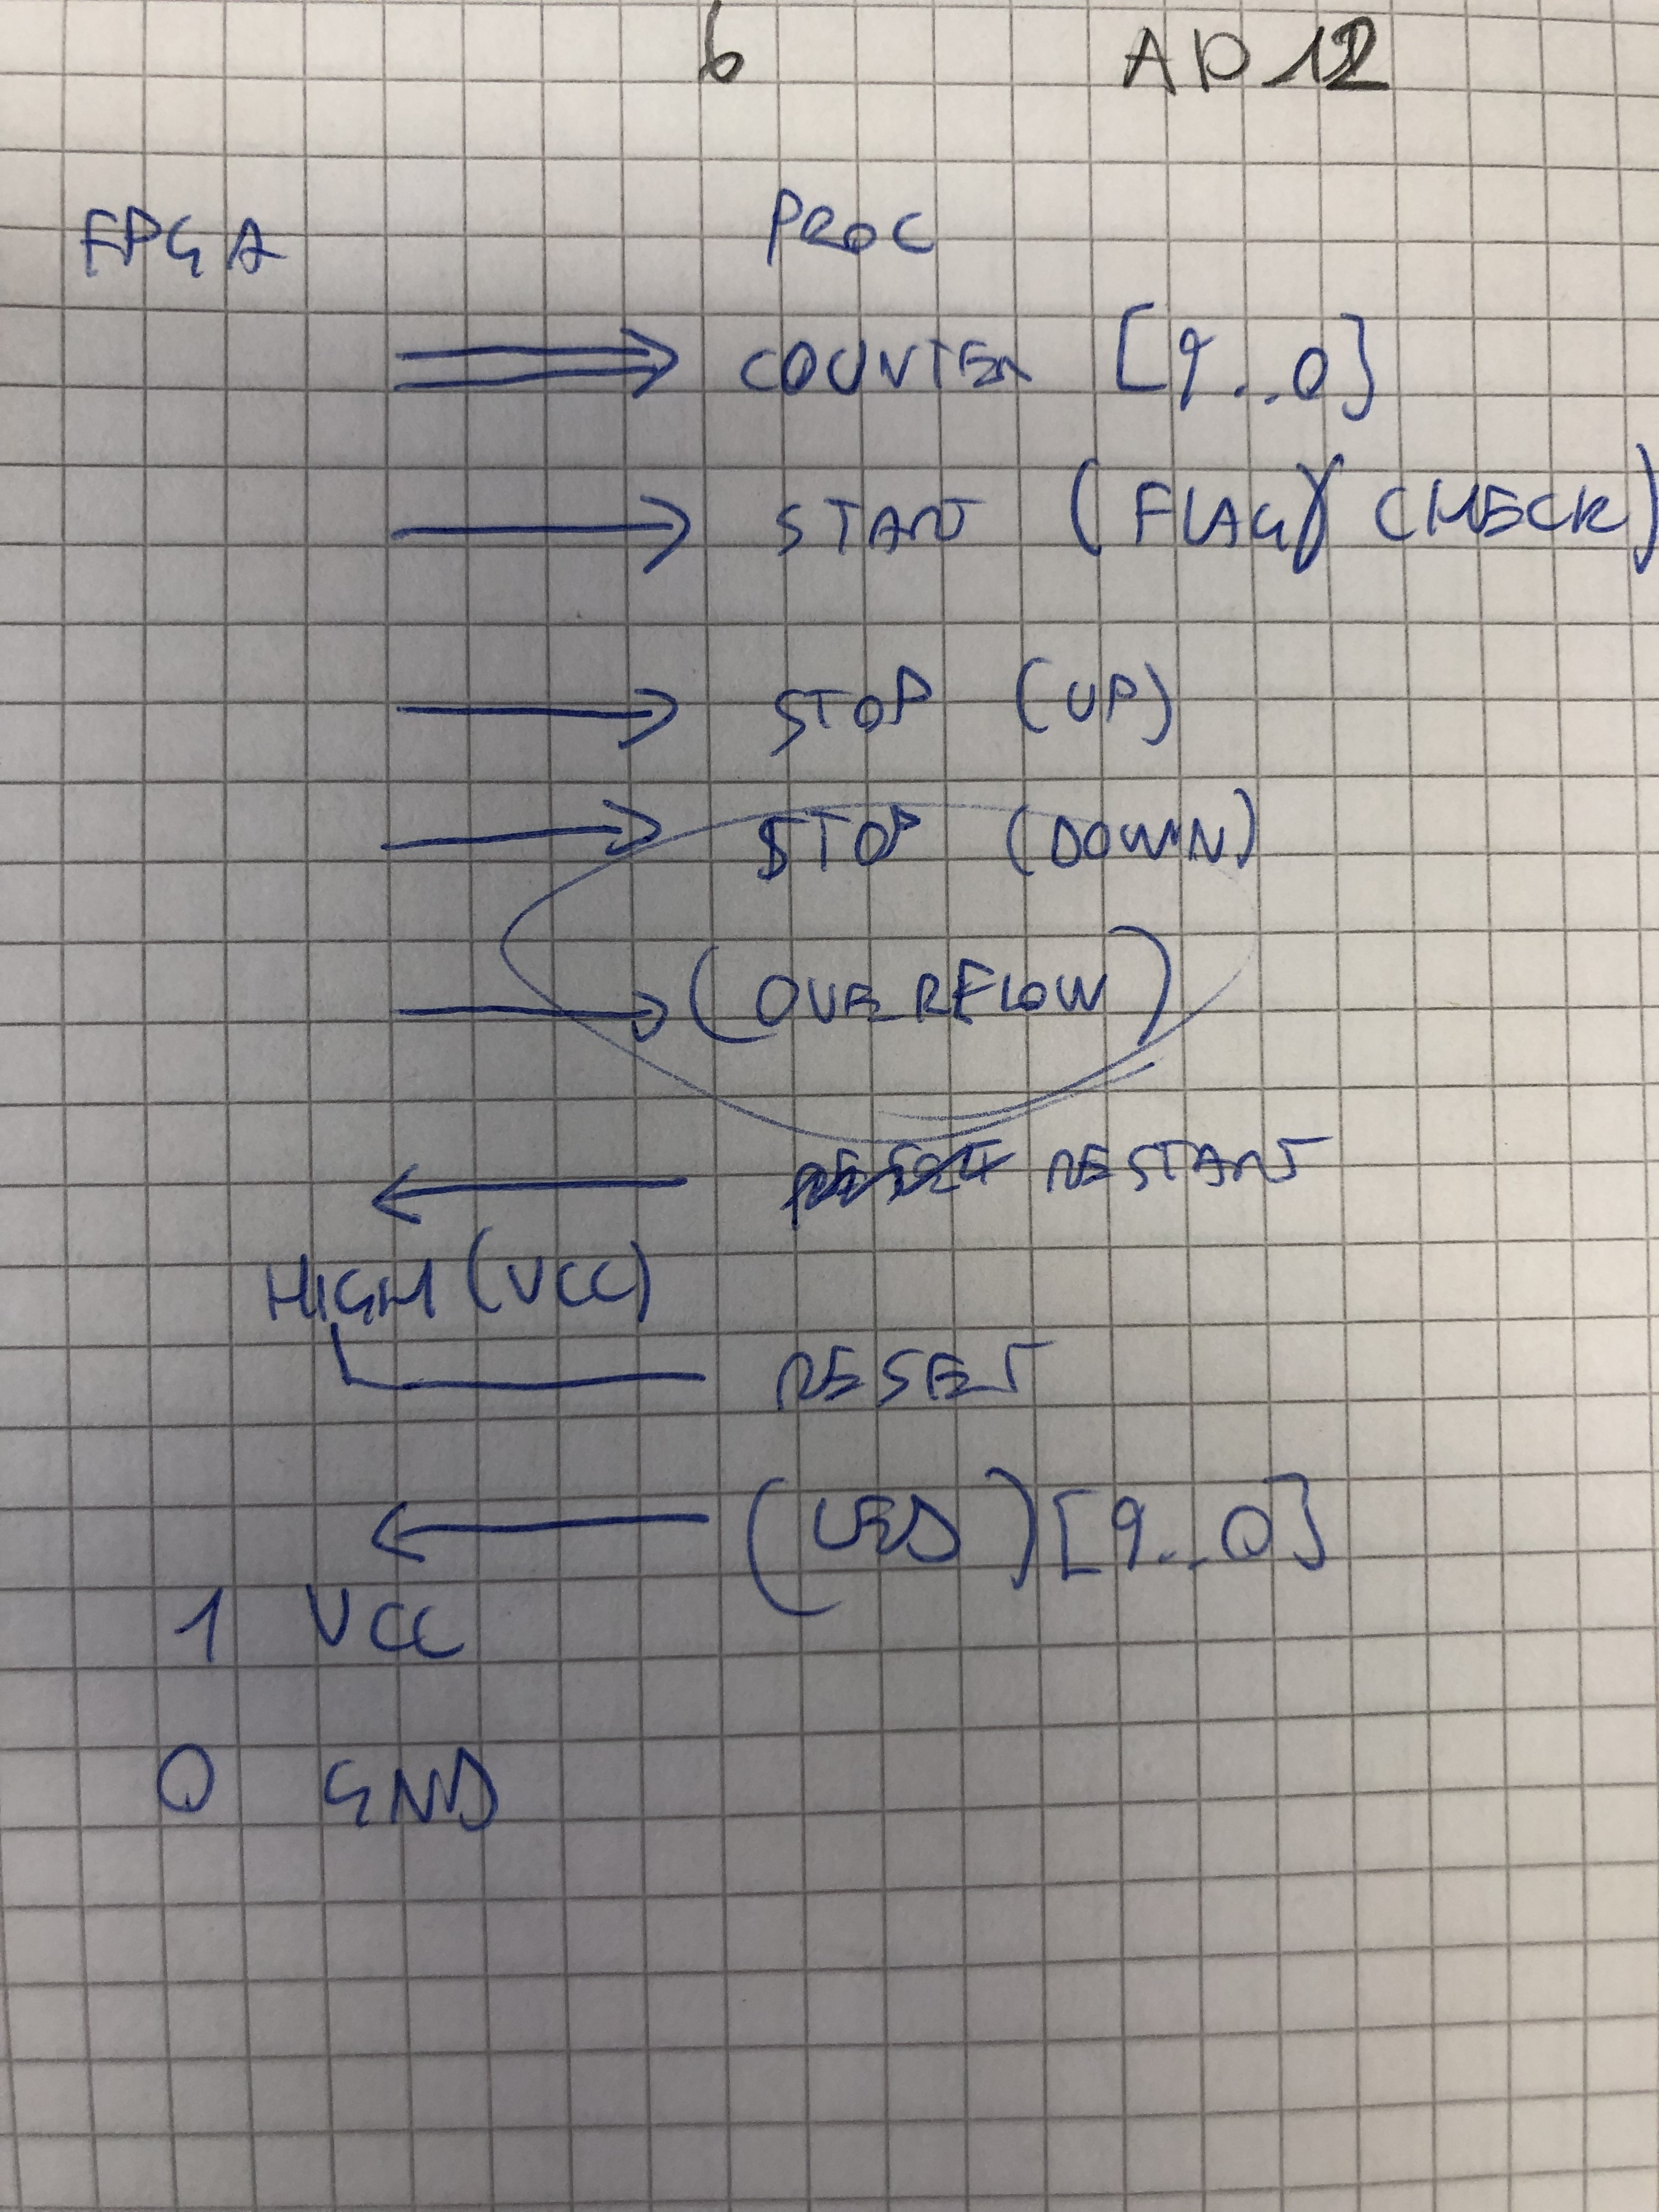
\includegraphics[scale=0.07]{Images/Schemas/Processeur.png}
        \end{figure}
        
        
    \item Pour la prochaine fois, il faut refaire les ports du processeurs. comme la photo du screenshot. Il faut aussi modifier le code avec nos noms de variable. J'ai refait le processeur avec Qsys ...vite fait controler et reconnecter les cables.
    \item AVANT DE LANCER LES LIGNES DE CODES DANS LE TERMINAL, (DAILLEUR LES LANCER UNE PAR UNE) NE PAS OUBLIER DE CREER UN DOSSIER ET DE TRAVAILLER DEDANS COMME C'EST ECRIT DANS LE FICHIER "INSTRUCTION.TXT"
    \item recontroler les noms des variables dans les fichier muon\_dac.c et muon\_daq.h sa doit etre le meme que les noms dans le processeur!
\end{itemize}

%%%%%%%%%%%%%%%%%%%%%%%%%%%%%%%%%%%%%%%%%%%%%%%%%%%%%%%%%%%%%%%%%
%%% 12.11.2018 %%%%%%%%%%%%%%%%%%%%%%%%%%%%%%%%%%%%%%%%%%%%%%%%%%
%%%%%%%%%%%%%%%%%%%%%%%%%%%%%%%%%%%%%%%%%%%%%%%%%%%%%%%%%%%%%%%%%

\section{\textbf{12.11.18}}
\begin{itemize}
    \item On a fini le code normalement tous devrait fonctionner....premiers résultats:\\
          20 61 ; 10 b8 ; 10 76 ; 10 81 ; 10 4a ; 10 ae ; 10 90 ; 10 0f ; 10 10 ; 20 37 ; 20 0f; 20 23 ; 10 4c ; 20 f3 ; 10 0c ; 20 c3 ; 10 61 ; 10 7a ; blablabla
    \item premier chiffre si c'est un up or down.
    \item A faire: ouverture + convertion des données 
\end{itemize}

\section{\textbf{17.12.18}}
Aujourd'hui Carmelo a tout effacé. Il faut encore tester avec le compteur en modulus 50 millions qui vas envoyé un signal sous forme de clock a chaque seconde ou deuxième compteur. Si ça marche pas, on doit débugger avec l'oscilloscope et si ça marche pas, on abandonne.


\section{\textbf{18.02.19}}

On a fait l'histogramme des mesures des oscillations/fluctuations sur un jour.
Conclusion: C'est que du bruit. On voulait mesurer une effet de fluctuation très petit (<1 pour cent) mais c'est un vieux équipement et on n'as pas calibrer pour le changement d'efficacité (efficiency) le long de la journée par exemple si il y a un changement de température.
Il faudrait faire une deuxième expérience a coté pour mesurer l'efficacité en fonction de la journée avec une source dont on connaît le nombre de particules par seconde.

\end{comment}

\end{document}